%% ============================================================================
%% Foundational NLP Tools for Ge'ez-Script Languages: A Systematic Review
%% Springer Nature sn-jnl rebuild (sn-mathphys-num, numbered references)
%% Compiler: lualatex + bibtex
%% ============================================================================

\documentclass[sn-mathphys-num]{sn-jnl}

\usepackage[numbers,sort&compress]{natbib}
\usepackage{graphicx}
\graphicspath{{../src/visualization/output/}}
\usepackage{multirow}
\usepackage{amsmath,amssymb,amsfonts}
\usepackage{amsthm}
\usepackage[title]{appendix}
\usepackage{xcolor}
\usepackage{textcomp}
\usepackage{manyfoot}
\usepackage{booktabs}
\usepackage{algorithm}
\usepackage{algorithmicx}
\usepackage{algpseudocode}
\usepackage{listings}
\usepackage{tabularx}
\usepackage{array}
\usepackage{longtable}
\usepackage{fontspec}
\usepackage{tikz}
\usetikzlibrary{shapes.geometric,arrows.meta,positioning}

%% Ragged-right flexible column for tabularx (avoids awkward justified
%% hyphenation breaks in narrow table cells, e.g. at page boundaries).
\newcolumntype{Y}{>{\raggedright\arraybackslash}X}

%% ----------------------------------------------------------------------
%% Ge'ez / Ethiopic script support (LuaLaTeX + fontspec)
%% Font confirmed installed and rendering real Ethiopic glyphs:
%%   Noto Sans Ethiopic (Regular + Bold), ~/.local/share/fonts/
%% ----------------------------------------------------------------------
\newfontfamily\geezfont{Noto Sans Ethiopic}
\newcommand{\geez}[1]{{\geezfont #1}}

%% ----------------------------------------------------------------------
%% Visually distinct VERIFY marker (red, bold) -- used ONLY for open
%% items that require author confirmation before submission. Not used
%% for any other purpose in this document.
%% ----------------------------------------------------------------------
\newcommand{\VERIFY}[1]{\textcolor{red}{\textbf{[VERIFY: #1]}}}

\theoremstyle{thmstyleone}
\newtheorem{theorem}{Theorem}
\newtheorem{proposition}[theorem]{Proposition}

\theoremstyle{thmstyletwo}
\newtheorem{example}{Example}
\newtheorem{remark}{Remark}

\theoremstyle{thmstylethree}
\newtheorem{definition}{Definition}

\raggedbottom

\begin{document}

\title[Foundational NLP Tools for Ge'ez-Script Languages]{Foundational NLP Tools for Ge'ez-Script Languages: A Systematic Tool-Centred Analysis}

\author*[1,2]{\fnm{Hailay Kidu} \sur{Teklehaymanot}}\email{teklehaymanot@l3s.de; hailaykidu.teklehaymanot@uzh.ch}

\author[3]{\fnm{Gebreagziher Gebrelibanos} \sur{Mesfun}}

\author[4]{\fnm{Tsegaye Semere} \sur{Gebremichael}}

\author[5]{\fnm{Gebrearegawi} \sur{Gebremariam}}

\author[6]{\fnm{Alemu Kumilachew} \sur{Tegegnie}}

\author[2]{\fnm{Nesina} \sur{Gr\"{u}tter}}

\affil*[1]{\orgdiv{L3S Research Center}, \orgname{Leibniz University Hannover}, \orgaddress{\city{Hannover}, \country{Germany}}}

\affil[2]{\orgname{University of Zurich}, \orgaddress{\city{Zurich}, \country{Switzerland}}}

\affil[3]{\orgname{Adigrat University}, \orgaddress{\city{Adigrat}, \country{Ethiopia}}}

\affil[4]{\orgname{National Tsing Hua University}, \orgaddress{\city{Hsinchu}, \country{Taiwan}}}

\affil[5]{\orgname{Axum University}, \orgaddress{\city{Axum}, \country{Ethiopia}}}

\affil[6]{\orgname{Bahir Dar University}, \orgaddress{\city{Bahir Dar}, \country{Ethiopia}}}

\abstract{The Ge'ez script is an ancient alphasyllabary used to write several languages of the Horn of Africa; this survey covers three of them: Amharic, Tigrinya, and Classical Ge'ez. Amharic and Tigrinya are spoken by tens of millions of people in Ethiopia and Eritrea. Classical Ge'ez is no longer spoken natively but is still used as the liturgical language of the Ethiopian and Eritrean Orthodox Tewahedo Churches and the Ethiopian and Eritrean Catholic Churches. Yet these languages remain underrepresented in natural language processing (NLP) research relative to their speaker population, reflecting a scarcity of foundational NLP tools, complex morphological structure, and limited digital infrastructure. This survey provides a systematic, tool-centred analysis organised around four methodological pillars: (i)~tokenisation and normalisation; (ii)~morphological analysis and synthesis; (iii)~text representation, embeddings, and evaluation; and (iv)~sequence labelling and structure extraction. We examine 69 individually live-verified publications from 2017 to 2026, in a review guided by PRISMA 2020, and report a 28-tool inventory of foundational tools, models, datasets, and linguistic resources independently confirmed publicly available on one of four repositories (GitHub, Zenodo, PyPI, HuggingFace) at the time of writing: 26 individually traceable to a specific paper within this corpus, plus two provenance-track additions (HornMorpho, MasakhaNER 1.0) whose originating papers fall outside the corpus. A dual inclusion standard governs the two halves of the survey: papers enter the literature corpus through a peer-review track or, if they release a concrete, checkable artefact, a provenance track, while tools enter the inventory on public provenance alone. Amharic is the most represented language in both the literature and the tool inventory, Tigrinya is second, and Classical Ge'ez is the least represented by both measures. Eight inventoried tools cover more than one of the three languages, but none is a script-level transfer framework designed for all three, and they follow no shared annotation or evaluation standard. This survey provides a PRISMA 2020 flow diagram, an aggregate characterisation of the reviewed literature, tool profiles with pillar classifications, a discussion of survey limitations, and seven research priorities derived from the gaps identified in the corpus.}

\keywords{Ge'ez script, low-resource NLP, morphologically rich languages, Amharic, Tigrinya, Classical Ge'ez, systematic review, PRISMA 2020, NLP tools, cross-lingual transfer}

\maketitle

\section{Introduction}\label{sec:intro}

Despite the transformative impact of deep learning, large-scale corpora, and multilingual models on NLP, only a small share of the world's 7,000+ languages are meaningfully represented in current language technologies \citep{joshi_state_2020}. Ge'ez-script languages remain underrepresented in this literature relative to their combined speaker population: Amharic and Tigrinya are spoken by tens of millions of people in Ethiopia and Eritrea, and Classical Ge'ez is retained today as the liturgical language of the Ethiopian and Eritrean Orthodox Tewahedo Churches and the Ethiopian and Eritrean Catholic Churches.

Contributing factors include limited funding for tool development, scarcity of digital corpora \citep{tonja_natural_2023}, and the computational demands of Semitic morphology combined with a non-Latin script \citep{teklehaymanot_movoc_2025}. The Ge'ez script's syllabic structure, which encodes consonant-vowel pairs as atomic \emph{fidels}, differs from Latin alphabets in ways that limit direct reuse of tokenisers and models built for alphabetic scripts \citep{teklehaymanot_tokenization_2025}.

\subsection*{Script Sample: A Shared Fidel Across Three Languages}

To illustrate the shared orthographic foundation that motivates this survey's cross-lingual framing, consider the Ge'ez fidel \geez{ሰላም} (\emph{sal\={a}m}, ``peace''), a lexical and orthographic cognate attested across all three languages under study:

\begin{itemize}
    \item Classical Ge'ez: \geez{ሰላም} (liturgical and historical usage)
    \item Amharic: \geez{ሰላም} (\emph{sälam})
    \item Tigrinya: \geez{ሰላም} (\emph{selam})
\end{itemize}

\noindent The identical fidel sequence across all three languages exemplifies both the opportunity (shared script structure enabling transfer learning, Section~\ref{sec:asymmetry}) and the challenge (a single tokeniser or embedding space must accommodate language-specific phonological and morphological divergence layered atop a common orthography) that motivate this survey's tool-centred, cross-lingual analysis.

\subsection{Motivation and Survey Scope}

This survey provides a systematic, tool-centred analysis of NLP research for Ge'ez-script languages. We organise the analysis around four methodological pillars: (1)~tokenisation and normalisation; (2)~morphological analysis and synthesis; (3)~text representation, embeddings, and evaluation; and (4)~sequence labelling and structure extraction.

Our approach is governed by an explicit \textbf{dual inclusion standard} (fully stated in Section~\ref{sec:dual-standard}): a systematic literature review of 69 individually live-verified papers (2017--2026) from major NLP venues and beyond, screened with guidance from PRISMA 2020 and using peer-review or (for a documented provenance-based subset) a concrete, verifiable tool/dataset contribution as the inclusion criterion. From this same corpus, we additionally report which of the papers' own tool, model, dataset, or resource contributions have an independently confirmed, currently live public release on GitHub, Zenodo, PyPI, or HuggingFace (Section~\ref{sec:tools-from-corpus}), keeping the two evidentiary standards -- peer-review-based literature inclusion, and provenance-based tool verification -- transparent and non-contradictory.

\subsection{Definition: Foundational NLP Tools}

For the purposes of this survey, we define \textbf{foundational NLP tools} as reusable, technically non-trivial software components that perform core NLP tasks essential for downstream language processing. Foundational tools are characterised by:

\begin{enumerate}
    \item \textbf{Core functionality:} Perform essential NLP operations (tokenisation, morphological analysis, embedding generation, sequence labelling) that enable more complex applications.
    \item \textbf{Reusability:} Designed as modular, deployable components that can be integrated into larger NLP pipelines or applications.
    \item \textbf{Language-specific design:} Incorporate knowledge of script structure (fidel-level encoding), morphological paradigms, or orthographic conventions unique to Ge'ez-script languages.
    \item \textbf{Technical non-triviality:} Require non-obvious algorithmic or engineering solutions beyond simple regex patterns or lookup tables.
    \item \textbf{Verifiable existence:} Published as open-source repositories, datasets, models, or papers with a stable, citable public identifier and clear provenance.
    \item \textbf{Production relevance:} Have demonstrated use in research applications, downstream systems, or academic projects, or show clear potential for practical deployment.
\end{enumerate}

We explicitly exclude: (i)~web applications or end-user software without published source code; (ii)~unpublished or proprietary tools without verifiable documentation; (iii)~simple heuristic scripts or ad hoc implementations; (iv)~tools designed exclusively for other scripts or language families, even if tangentially applied to Ge'ez languages. This definition restricts the inventory to reproducible, shareable infrastructure, independent of whether that infrastructure has been peer-reviewed (see Section~\ref{sec:dual-standard}).

\subsection{Key Contributions}

\begin{enumerate}
    \item Systematic tool-centred analysis of foundational Ge'ez-script NLP tools across three Ge'ez-script languages (Amharic, Tigrinya, Classical Ge'ez) and four methodological pillars.
    \item Comprehensive literature review of 69 individually live-verified papers (2017--2026) guided by PRISMA 2020, including a PRISMA flow diagram and an aggregate characterisation of the reviewed literature (Section~\ref{sec:prisma}).
    \item An explicit, transparent dual inclusion standard reconciling peer-review-based literature screening with provenance-based tool-inventory criteria (Section~\ref{sec:dual-standard}).
    \item Quantified evidence of research asymmetry, computed directly from the verified corpus: Amharic is the most represented language in both the literature (68\% of 69 papers) and the tool inventory (79\% of 28 tools), Tigrinya is second in both, and Classical Ge'ez remains the least represented in both and critically underserved.
    \item A tool inventory of 28 foundational tools, models, datasets, and linguistic resources independently confirmed publicly available on GitHub, Zenodo, PyPI, or HuggingFace (Section~\ref{sec:tools-from-corpus}): 26 individually traceable to a specific paper in the 69-paper corpus, plus two provenance-track additions (HornMorpho, MasakhaNER 1.0); pillar counts and language coverage are tallied directly from that verified table.
    \item Explicit reporting of Pillar 4 (sequence labelling) resources: 3 tools have an independently confirmed public repository (2 corpus-traceable, 1 provenance-track); further sequence-labelling artefacts are described in the literature but lack a confirmable public release and are reported as such rather than counted.
    \item Script-level transfer learning identified as an ad hoc and undocumented avenue requiring coordinated development and shared standards.
    \item Seven-priority research agenda grounded in systematic evidence for future tool development, including an explicit call for independent data-quality assessment of the catalogued datasets and tools, and for deliberate reuse of classical Semitic studies and digital-humanities resources (Section~\ref{sec:agenda}).
\end{enumerate}

\section{Methodology}\label{sec:methodology}

We conducted a systematic literature review guided by the PRISMA 2020 guidelines \citep{page_prisma_2021}, complemented by parallel tool discovery across multiple repositories governed by a separate, explicitly stated provenance standard.

\subsection{Literature Search Strategy}\label{sec:literature-search}

The literature search began with systematic searches across six major peer-reviewed NLP venues: ACL, EMNLP, NAACL, LREC, COLING, and EACL, using search terms that combined language names (Amharic, Tigrinya, Ge'ez), script designations (Ethiopic, Fidel), and NLP task labels corresponding to all four methodological pillars (tokenisation and normalisation; morphological analysis and synthesis; embeddings and language models; part-of-speech tagging, named entity recognition, and parsing), supplemented by forward and backward citation tracing. This six-venue search is the primary channel for the peer-reviewed track of the dual inclusion standard (Section~\ref{sec:dual-standard}) and, on its own, is where the large majority of the corpus's core NLP-conference contributions were found. It is deliberately not the corpus's only source: consistent with the dual inclusion standard, the search was extended to (a)~other peer-reviewed venues outside the six named ones (e.g.\ \emph{Information}, \emph{PLOS ONE}, \emph{Language Resources and Evaluation}, ACM and IEEE conference proceedings, and regional venues such as RAIL, AfricaNLP, and ICT4DA) whenever a paper independently satisfied the peer-review and scope criteria below, and (b)~non-peer-reviewed preprints and workshop papers admitted specifically under the provenance-based track described in Section~\ref{sec:dual-standard}, where the paper describes a concrete, independently verifiable tool, dataset, or corpus for a Ge'ez-script language. Of the 69 papers in the final corpus, 18 were published at the six named venues; the remaining 52 were found via this extended, dual-standard-governed search and were individually live-verified before inclusion. Of those 52, 35 appeared at other peer-reviewed or workshop venues (e.g.\ ACM SIGAPP, ACM SIGIR, \emph{ACM TALLIP}, PLOS ONE, \emph{Information}, \emph{Language Resources and Evaluation}, NeurIPS Datasets \& Benchmarks, IEEE and Springer proceedings, RAIL, AfricaNLP, WiNLP, ICT4DA) and were admitted under the peer-review track; the other 16 are preprint- or repository-only records admitted under the provenance track (Section~\ref{sec:dual-standard}). These three figures (18, 35, 16) are tallied directly from the \texttt{Venue} and \texttt{Venue\_Type} columns of \texttt{data/verified\_papers\_live\_search.csv} and sum to 69.

\textbf{Search period, sources, and terms.} The literature search and screening were carried out between July and mid-September 2026. The corpus was first recorded on 16 September 2026 (71 records); full-text re-checking then excluded one record (MasakhaPOS, in which Amharic is not a subject of the work; Section~\ref{sec:tools-from-corpus}), leaving 70; one further record (P046), withdrawn by its authors, was removed during revision, leaving 69. All bibliographic details and repository links were verified on 21 September 2026. Publications appearing up to the closing date of 16 September 2026 were eligible. Searches targeted the six core venues above, were extended to other peer-reviewed venues and regional workshops, and were supplemented by forward and backward citation tracing from included papers. Queries combined a language name (Amharic, Tigrinya, Ge'ez) or script designation (Ethiopic, Fidel) with NLP task labels covering the four pillars (e.g.\ tokenisation, normalisation, morphological analysis, morphological synthesis, embeddings, language models, part-of-speech tagging, named entity recognition, parsing). The search was conducted manually and no query-level log was preserved; stage counts are therefore reported only where they are documented (Section~\ref{sec:prisma-flow}).

\textbf{Inclusion criteria (literature review, peer-review track):} Peer-reviewed publications (journal articles and conference/workshop proceedings, from the six named venues or elsewhere) describing foundational NLP tools, datasets, or algorithms for Ge'ez-script languages, published 2016--2026, with Amharic, Tigrinya, and/or Classical Ge'ez as an actual subject of the work rather than an incidental member of a large, undifferentiated multilingual set.

\textbf{Inclusion criteria (literature review, provenance track):} Non-peer-reviewed preprints or workshop papers are additionally eligible, under the same year and language-focus requirements above, if and only if the paper describes a concrete, independently checkable tool, dataset, corpus, or software pipeline for a Ge'ez-script language (Section~\ref{sec:dual-standard}); topical relevance alone is not sufficient grounds for admission under this track.

\textbf{Exclusion criteria (literature review):} Grey literature without an identifiable, checkable artefact; downstream applications that contribute no tool, dataset, or algorithm of their own (application papers that do release such a contribution, e.g.\ a speech or OCR dataset, are in scope); papers published outside 2016--2026; and papers whose treatment of Amharic, Tigrinya, or Classical Ge'ez is not independently identifiable (e.g.\ general multilingual-NLP or general machine-learning papers included only because they are widely cited, not because they study a Ge'ez-script language).

\textbf{Peer-review-track papers outside the six named venues.} Thirty-five peer-reviewed or workshop papers meeting the full inclusion criteria were published outside the six named venues, across journals (\emph{ACM TALLIP}, PLOS ONE, \emph{Information}, \emph{Language Resources and Evaluation}, \emph{Ethiopian Journal of Science and Sustainable Development}, among others), ACM, IEEE and Springer conference proceedings, and regional or topical workshops (RAIL, AfricaNLP, WiNLP, ICT4DA, LT4All). Two representative examples are Gezmu et al.'s portable Amharic spelling corrector (LREC 2018) \citep{gezmu_portable_2018} and Alemneh et al.'s dictionary-based Amharic sentiment lexicon (ICT4DA 2019) \citep{alemneh_dictionary_2019}; the full list is given in Appendix~\ref{app:corpus-list}, and the count is tallied directly from the CSV's \texttt{Venue} column.

\textbf{Provenance-track papers.} Consistent with the dual inclusion standard (Section~\ref{sec:dual-standard}), sixteen papers that were available only as preprints or repository records at the closing date were admitted under the provenance track (this track admits \emph{papers} and is distinct from the provenance-based standard for the tool inventory, Section~\ref{sec:tool-inventory}). Seven describe a concrete released artefact: AmQA \citep{abedissa_amqa_2023}, the Amharic Whisper fine-tuning and evaluation data \citep{gete_whispering_2025}, the TLMD corpus \citep{gaim_tlmd_2021}, an Amharic news classification dataset \citep{azime_amharic_2021}, the VEXMLM vocabulary-extended model \citep{teklehaymanot_expanding_2026}, an adapted TrOCR model for printed Tigrinya \citep{medhanie_adapting_2026}, and a Ge'ez numeral image dataset \citep{beyene_handwritten_2019}. Five have since appeared in peer-reviewed venues and are cited in their published form \citep{teklehaymanot_lowresource_2025,yimer_learning_2024,gashaw_amharicarabic_2019,gondere_handwritten_2019,adnew_semantically_2024}. Two were recorded on this track conservatively although they had already been peer-reviewed \citep{yimam_introducing_2021,kidane_exploration_2021}. The remaining two, a survey of Tigrinya NLP \citep{gaim_tigrinya_2025} and a study of Ge'ez machine translation \citep{wassie_machine_2023}, describe no released artefact and so do not strictly meet this track's criterion; they are retained as two of the very few studies of Tigrinya and Classical Ge'ez respectively, and contribute to no tool count.

This yields a final literature corpus of \textbf{69} papers (2017--2026; no eligible pre-2016 candidate met the language-focus criterion). Every paper is individually verified (title, authors, venue, and DOI/URL), and the corpus composition, pillar classification, and inclusion rationale for each entry are reconciled against the dual inclusion standard of Section~\ref{sec:dual-standard}.

\subsection{An Explicit Dual Inclusion Standard}\label{sec:dual-standard}

A methodology that screens literature by peer-review status while simultaneously harvesting tools from GitHub, Zenodo, PyPI, and HuggingFace---platforms that are, by definition, grey literature or non-peer-reviewed---would be internally contradictory if left unstated. Several artefacts in this survey make the tension concrete: MoVoC and the LGSE Project each have a peer-reviewed publication (EMNLP 2025 Findings and LREC 2026 respectively; \citealp{teklehaymanot_movoc_2025,teklehaymanot_lgse_2026}) but no independently confirmable public release of the artefact each paper reports, whereas HornMorpho is a public, actively maintained repository whose originating publication \citep{gasser_hornmorpho_2011} falls outside this survey's review window; a tool's practical existence and its peer-review status are independent properties, general to this survey's scope. To resolve this transparently rather than silently, we adopt \textbf{two distinct, explicitly declared inclusion standards} for the two halves of this survey:

\begin{itemize}
    \item \textbf{Literature review standard (two tracks):} Applies to the literature corpus analysed in Section~\ref{sec:prisma}. A paper is admitted either through the \emph{peer-review track} (journal articles and conference/workshop proceedings) or through the \emph{provenance track}, which admits a non-peer-reviewed paper only if it describes a concrete, independently checkable tool, dataset, corpus, or software pipeline for a Ge'ez-script language (Section~\ref{sec:literature-search}). Each paper's track is recorded in the corpus file, so the two groups can always be reported separately. Related Work (Section~\ref{sec:related}) may additionally cite background sources outside the corpus.
    \item \textbf{Tool-inventory standard (provenance-based):} Applies exclusively to the tool inventory (Section~\ref{sec:tool-inventory} onward). Any artefact---code repository, dataset, or model---with a \emph{stable, versioned, citable public identifier} (a DOI, a GitHub commit/release tag, a HuggingFace model card, or a Zenodo record) is eligible for the tool inventory \emph{regardless of peer-review status}. Peer review is not required for tool-inventory inclusion because the inventory documents publicly released tools regardless of whether they were ever submitted for academic review.
\end{itemize}

These two standards are deliberately different and are never merged: a count of ``peer-reviewed papers'' and a count of ``inventoried tools'' answer different questions and should not be added together or used to validate one another. Every place in this manuscript that reports a count is labelled with which standard produced it.

\textbf{The standard in practice.} Applying the literature-review standard above, no candidate that is not specifically about a Ge'ez-script language is admitted to the literature corpus, and no preprint is admitted on topical relevance alone, regardless of the work's practical importance elsewhere in NLP (e.g.\ foundational architecture papers such as \emph{Attention Is All You Need} are correctly excluded from the literature-review corpus, since they are not about a Ge'ez-script language, irrespective of their citation count or influence). This is the same asymmetry the dual standard is designed to make legible: a tool or model can be practically significant and provenance-verifiable (and thus eligible for the tool inventory) without being an included item in the literature corpus, and vice versa. The provenance track of the literature standard and the provenance-based tool-inventory standard are distinct: the former admits a \emph{paper} that describes an artefact, the latter admits an \emph{artefact} with a public identifier.

\textbf{What ``verified'' does and does not mean in this survey.} Throughout this manuscript, an entry is described as ``verified'' when its bibliographic details (title, authors, venue, year, DOI/URL) or, for the tool inventory, its public repository link (Section~\ref{sec:tool-discovery}), were independently confirmed to exist and to match what the source paper reports. This is existence and provenance verification, not data-quality assessment: this survey does not re-annotate, audit, or independently measure the accuracy, inter-annotator agreement, label correctness, or cleanliness of any dataset it catalogues. The corpus's only quality signal is indirect -- whether the paper describing a dataset passed peer review (Section~\ref{sec:dual-standard}) or, for provenance-track artefacts, whether it carries a stable public identifier -- and neither of these is equivalent to an independent quality audit of the data itself. A peer-reviewed venue may or may not have required rigorous annotation-quality reporting (e.g.\ inter-annotator agreement) as a condition of acceptance, and this survey did not separately check. Readers intending to build on any dataset or tool catalogued here should treat its quality as unassessed by this survey and consult the source paper's own reported quality-control methodology (where available) before use; this gap is discussed further in Section~\ref{sec:limitations} and named as a research priority in Section~\ref{sec:agenda}.

\subsection{Tool Discovery and Verification}\label{sec:tool-discovery}

For every paper in the 69-paper verified literature corpus that reports creating a tool, model, dataset, or other resource (identified from the paper's own stated contribution), we searched for an independently checkable public release of that specific artefact on one of four repositories, applying the provenance-based standard defined in Section~\ref{sec:dual-standard}:

\begin{itemize}
    \item \textbf{GitHub:} Open-source code repositories.
    \item \textbf{Zenodo:} Academic datasets and models with assigned DOIs.
    \item \textbf{PyPI:} Python package ecosystem.
    \item \textbf{HuggingFace Hub:} Pre-trained models and datasets with model/dataset cards.
\end{itemize}

\noindent An artefact is counted as verified only when a live, resolvable link to \emph{that specific artefact} was found and confirmed during this search, matching what the paper itself reports; a link that resolves to a different, later, or otherwise non-matching artefact does not satisfy this standard, even if it is publicly hosted under the same author's account. An artefact is excluded from the verified count whenever no such link could be independently confirmed, even where the source paper itself asserts a public release. This yielded 26 of the tools reported in Section~\ref{sec:tools-from-corpus} and Table~\ref{table:tools-from-corpus}, each traceable to a specific paper in the literature corpus. This corpus-first search is a deliberate scope limitation, not a claim that no other public Ge'ez-script NLP tool exists: Table~\ref{table:tools-from-corpus} additionally documents two provenance-track tools found outside this search (HornMorpho, MasakhaNER 1.0; see the note following that table), bringing the inventory to 28 tools in total.

\textbf{Automated link verification.} Every repository cell in Table~\ref{table:tools-from-corpus} is an exact, individually-resolved identifier (organisation/repository for GitHub, exact model or dataset slug for HuggingFace, DOI for Zenodo), not a platform name alone. This is checked programmatically by the committed script \texttt{src/verification/check\_tool\_links.py}, which issues a live HTTP or platform-API request against each repository link in the table and writes a timestamped log to \texttt{src/verification/output/tool\_link\_check.txt}. Where the platform's API is reachable and not rate-limited, the log additionally records a resolved commit SHA or dataset revision hash; GitHub's unauthenticated API is rate-limited to 60 requests/hour, so a run against all links may report some GitHub entries as resolved without a SHA (recorded as such in the log) rather than fail outright. The inventory is frozen at its verification date, 21 September 2026: on that date every link in the table resolved, and releases that appear afterwards are recorded in the repository file \texttt{data/tool\_inventory\_addenda.csv} but not counted here (see the committed log for per-entry status, SHA where available, and access timestamp); this check can be independently reproduced with \texttt{python -m src.verification.check\_tool\_links}.

\section{Related Work}\label{sec:related}

This systematic review is positioned within three complementary research streams.

\subsection{Low-Resource Language NLP}

The scarcity of NLP infrastructure for Ge'ez-script languages reflects broader patterns in low-resource language technology. Joshi et al.\ \citep{joshi_state_2020} document linguistic diversity gaps in NLP research, including the underrepresentation of African languages. Blodgett et al.\ \citep{blodgett_language_2021} analyse power imbalances and bias in NLP systems, connecting tool scarcity to linguistic inequality. This survey quantifies the equivalent gap for the Ge'ez-script language family specifically: which tools exist, for which languages, and with what provenance.

\subsection{Ge'ez-Script NLP and Script-Aware Methods}

Recent work has begun addressing Ge'ez-script-specific challenges. Gaim \& Park \citep{gaim_tigrinya_2025} provide a comprehensive survey of Tigrinya NLP, characterising the state of the art across 15 downstream tasks including morphological processing, part-of-speech tagging, named entity recognition, machine translation, and question answering. Tonja et al.\ \citep{tonja_natural_2023} survey NLP challenges and opportunities across four Ethiopian languages (Amharic, Afaan Oromo, Tigrinya, and Wolaytta), consolidating scattered resources into a centralised repository. Neither survey reports a tool inventory scoped specifically to the three languages sharing the Ge'ez script and cross-checked against live repository sources, which is the contribution of the present work.
The LGSE Project \citep{teklehaymanot_lgse_2026} develops lexically grounded subword embedding initialisation for low-resource language adaptation across Amharic and Tigrinya; it is peer-reviewed (LREC 2026) and is therefore part of the literature corpus, but no live public repository of its released embeddings could be independently confirmed, so it is \emph{not} counted among the verified tools in Table~\ref{table:tools-from-corpus} (Section~\ref{sec:asymmetry}). MoVoC \citep{teklehaymanot_movoc_2025} integrates morphology-aware subword construction for Ge'ez-script languages and is likewise peer-reviewed (EMNLP 2025 Findings). Mekonnen et al.\ \citep{mekonnen_optimized_2025} contribute text-embedding models and benchmarks for Amharic passage retrieval, reporting dense-retrieval results above multilingual baselines at a smaller parameter count. The EthioLLM initiative \citep{tonja_ethiollm_2024} pre-trains language models across five Ethiopian languages; it is peer-reviewed (LREC-COLING 2024; ACL Anthology \texttt{2024.lrec-main.561}) and is included in the literature corpus under the peer-review track of Section~\ref{sec:dual-standard}.

\subsection{Survey Methodology and PRISMA 2020 Standards}

This systematic review is guided by the PRISMA 2020 guidelines \citep{page_prisma_2021}, which supersede the earlier PRISMA-P (2015) guidance---PRISMA-P being intended specifically for review \emph{protocols} (pre-registration documents) rather than for reporting completed systematic reviews. Adapting systematic review methodology from medical/health research to NLP, the dual approach described in Section~\ref{sec:dual-standard}---combining peer-reviewed literature with tool discovery across multiple repositories---extends traditional surveys by capturing both documented (published) and emerging (tool-repository) artefacts. This reveals a structural gap: many tools developed at scale lack academic publication, and many academic contributions lack maintained, discoverable code. Bridging this publication-implementation gap is a key motivation for the seven-priority research agenda (Section~\ref{sec:agenda}).

\section{Systematic Literature Review: PRISMA 2020 Analysis}\label{sec:prisma}

This section reports the results of the literature screening process described in Section~\ref{sec:literature-search}, together with an aggregate characterisation of the included corpus.

\subsection{PRISMA 2020 Flow Diagram}\label{sec:prisma-flow}

Figure~\ref{fig:prisma-flow} presents the screening process in the standard PRISMA 2020 four-stage layout (Identification, Screening, Eligibility, Included). Consistent with this survey's evidence-only standard, exact counts are shown only for the stages that are independently verifiable against a preserved, checkable artefact: the 71 records assessed in full text, of which two were excluded (MasakhaPOS, Section~\ref{sec:tools-from-corpus}; and P046, withdrawn by its authors), and the \textbf{69} papers in the final included corpus, each individually confirmed against \texttt{data/verified\_papers\_live\_search.csv} (title, authors, venue, and DOI/URL verified per entry; Section~\ref{sec:literature-search}). Counts for the Identification and Screening stages (records identified, duplicates removed, records screened) are not shown, because no preserved search log exists from which to derive them; presenting invented figures for these stages -- even if visually conventional for a PRISMA diagram -- would not meet this survey's traceability standard. Each intermediate box instead names the screening step actually performed (Section~\ref{sec:literature-search}), without an accompanying count.

\begin{figure}[h]
\centering
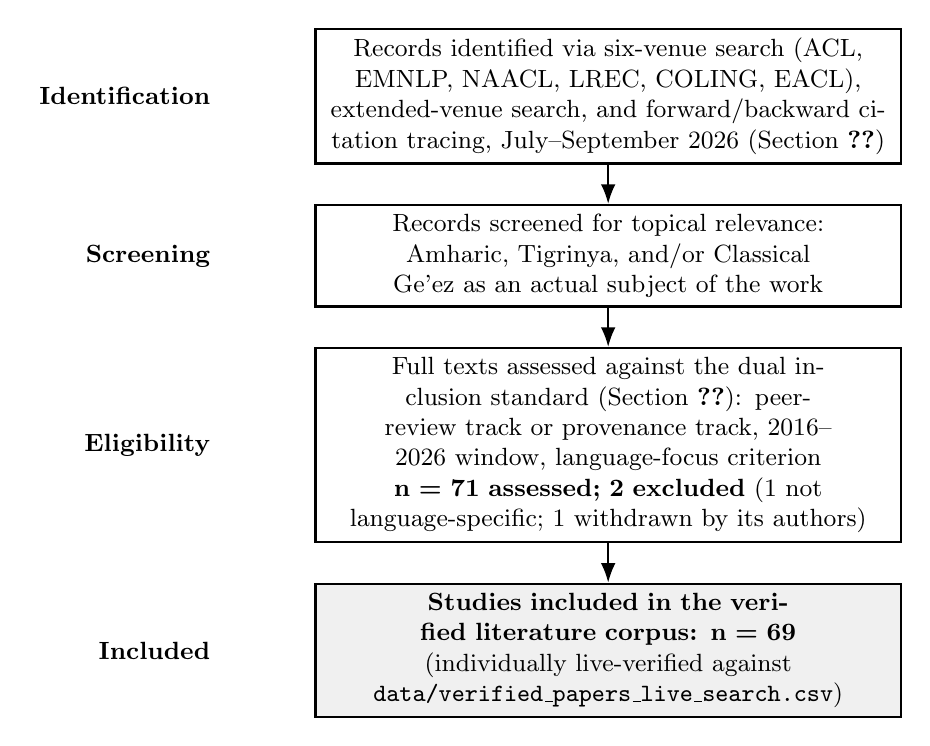
\begin{tikzpicture}[
  node distance=0.5cm and 1.2cm,
  box/.style={rectangle, draw, thick, text width=7.2cm, align=center, minimum height=1.1cm, font=\small},
  finalbox/.style={rectangle, draw, thick, fill=gray!12, text width=7.2cm, align=center, minimum height=1.1cm, font=\small},
  stagelabel/.style={font=\bfseries\small, text width=2.2cm, align=right},
  arr/.style={-{Latex[length=2.5mm]}, thick}
]
  \node[box] (identified) {Records identified via six-venue search (ACL, EMNLP, NAACL, LREC, COLING, EACL), extended-venue search, and forward/backward citation tracing, July--September 2026 (Section~\ref{sec:literature-search})};
  \node[stagelabel, left=of identified] (lab1) {Identification};

  \node[box, below=of identified] (screened) {Records screened for topical relevance: Amharic, Tigrinya, and/or Classical Ge'ez as an actual subject of the work};
  \node[stagelabel, left=of screened] (lab2) {Screening};

  \node[box, below=of screened] (eligibility) {Full texts assessed against the dual inclusion standard (Section~\ref{sec:dual-standard}): peer-review track or provenance track, 2016--2026 window, language-focus criterion \\ \textbf{n = 71 assessed; 2 excluded} (1 not language-specific; 1 withdrawn by its authors)};
  \node[stagelabel, left=of eligibility] (lab3) {Eligibility};

  \node[finalbox, below=of eligibility] (included) {\textbf{Studies included in the verified literature corpus: n = 69} \\ \small (individually live-verified against \texttt{data/verified\_papers\_live\_search.csv})};
  \node[stagelabel, left=of included] (lab4) {Included};

  \draw[arr] (identified) -- (screened);
  \draw[arr] (screened) -- (eligibility);
  \draw[arr] (eligibility) -- (included);
\end{tikzpicture}
\caption{PRISMA 2020 flow diagram for the systematic literature review. Exact counts are reported only for the stages documented in the repository's version history: 71 records assessed in full text, 2 excluded, and $n=69$ included (\texttt{data/verified\_papers\_live\_search.csv}). No preserved search log exists to support counts at the Identification or Screening stages, so none are asserted.}\label{fig:prisma-flow}
\end{figure}

\noindent The final included-studies count ($n=69$) shown in Figure~\ref{fig:prisma-flow} is an exact count of the individually live-verified papers in \texttt{data/verified\_papers\_live\_search.csv} (title, authors, venue, and DOI/URL independently confirmed for every entry), not an aggregate estimate. Should a preserved search log become available for the Identification, Screening, or Eligibility stages, exact counts can be added to Figure~\ref{fig:prisma-flow} at that time; until then, this survey reports only what can be independently verified.

\subsection{Aggregate Characterisation of the Reviewed Literature}\label{sec:prisma-characterisation}

The following is an aggregate characterisation of the 69 included studies, tallied directly from \texttt{data/verified\_papers\_live\_search.csv}. It is explicitly \emph{not} a per-paper bibliography or itemised list; rather, it summarises distributional patterns across the corpus as a whole.

\begin{table}[h]
\caption{Characterisation of the reviewed literature ($n=69$) by language focus, tallied directly from the verified corpus. Percentages sum to more than 100\% because multi-language studies (e.g., papers covering Amharic and Tigrinya jointly) are counted under each language they address.}\label{table:lit-by-language}
\begin{tabular}{@{}lcc@{}}
\toprule
\textbf{Language focus} & \textbf{Studies} & \textbf{\% of 69} \\
\midrule
Amharic & 47 & 68\% \\
Tigrinya & 26 & 38\% \\
Classical Ge'ez & 14 & 20\% \\
\botrule
\end{tabular}
\end{table}

\begin{table}[h]
\caption{Characterisation of the reviewed literature ($n=69$) by methodological pillar, tallied directly from the verified corpus.}\label{table:lit-by-pillar}
\begin{tabular}{@{}lcc@{}}
\toprule
\textbf{Pillar} & \textbf{Studies} & \textbf{\% of 69} \\
\midrule
P1: Tokenisation and normalisation & 1 & 1\% \\
P2: Morphological analysis and synthesis & 3 & 4\% \\
P3: Embeddings, language models, and evaluation & 33 & 48\% \\
P4: Sequence labelling and structure extraction & 6 & 9\% \\
Other / infrastructure and resource papers & 26 & 38\% \\
\botrule
\end{tabular}
\end{table}

\begin{table}[h]
\caption{Characterisation of the reviewed literature ($n=69$) by publication year, grouped into three-year bands (2016--2026), tallied directly from the verified corpus.}\label{table:lit-by-year}
\begin{tabular}{@{}lcc@{}}
\toprule
\textbf{Period} & \textbf{Studies} & \textbf{\% of 69} \\
\midrule
2016--2018 & 5 & 7\% \\
2019--2021 & 23 & 33\% \\
2022--2024 & 27 & 39\% \\
2025--2026 & 14 & 20\% \\
\botrule
\end{tabular}
\end{table}

\noindent Tables~\ref{table:lit-by-language}--\ref{table:lit-by-year} are exact tallies computed directly from \texttt{data/verified\_papers\_live\_search.csv} (the 69-paper corpus). Amharic is substantially more represented than Tigrinya in the literature corpus (68\% vs.\ 38\% of papers, overlapping count); Classical Ge'ez is the least-represented language (20\%), consistent with the tool-inventory findings. The pillar distribution shows a pronounced concentration in P3 (embeddings, language models, and evaluation; 48\%) and Other/infrastructure (38\%), with P1 (tokenisation, 1\%) and P2 (morphology, 4\%) markedly underrepresented in the literature relative to their conceptual centrality to Ge'ez-script NLP -- a gap discussed further in Section~\ref{sec:limitations}. The timeline shows publication activity concentrated in 2022--2026 (59\% of the corpus), consistent with the broader growth of multilingual and African-language NLP research documented by \citet{joshi_state_2020}.

\textbf{Reconciliation.} Every count in Table~\ref{table:lit-by-year} and Figure~\ref{fig:temporal-dist} is generated from the same single source of truth, \texttt{data/verified\_papers\_live\_search.csv}, by the committed script \texttt{src/visualization/generate\_verified\_corpus\_charts.py}. Per-year counts are 2017:\,1, 2018:\,4, 2019:\,6, 2020:\,7, 2021:\,10, 2022:\,9, 2023:\,6, 2024:\,12, 2025:\,8, 2026:\,6, summing to 69 and grouping to the 5/23/27/14 bands reported in Table~\ref{table:lit-by-year}. This reconciliation is not asserted from prose alone: the committed script \texttt{src/verification/check\_figures\_match\_csv.py} (i)~recomputes these values directly from the CSV, (ii)~regenerates all four figures and asserts byte-for-byte equality against the committed PNGs, (iii)~extracts every image embedded in the compiled \texttt{manuscript.pdf} and asserts a pixel-identical match to each committed PNG, and (iv)~parses Table~\ref{table:tools-from-corpus} directly and asserts the pillar and artefact-type prose elsewhere in this manuscript matches the table's own columns. The script exits non-zero on any mismatch; its output is committed at \texttt{src/verification/output/figures\_and\_tables\_check.txt} and was all-passing immediately before this submission. Reproduce with \texttt{python -m src.verification.check\_figures\_match\_csv}.

\subsection{Foundational Tools Identified Directly from the Reviewed Papers}\label{sec:tools-from-corpus}

This subsection builds the survey's single tool inventory, discussed further in Section~\ref{sec:tool-inventory}: it identifies how many artefacts the 69 reviewed papers themselves report creating that also have an independently verifiable public release on one of the four repositories (GitHub, Zenodo, PyPI, HuggingFace), then adds the small number of provenance-track tools found outside the corpus under the standard of Section~\ref{sec:dual-standard}. There is one inventory and one table (Table~\ref{table:tools-from-corpus}); Section~\ref{sec:tool-inventory} presents and discusses its results rather than deriving a second, independent count.

Every paper in the corpus records, in \texttt{data/verified\_papers\_live\_search.csv}, how many tools, datasets, and models it reports as its own contribution (the \texttt{Tools\_Count}, \texttt{Datasets\_Count}, and \texttt{Models\_Count} fields). Summed directly across the 69 reviewed papers, these fields name \textbf{75 artefacts across 53 papers}; this is a mechanical tally of what each paper's own count fields state; it is not filtered by whether an artefact plausibly meets this survey's foundational-tool definition (Section~\ref{sec:tool-inventory}), so it is an upper bound, not the number of artefacts assessed as in-scope. Of these, \textbf{26 artefacts from 17 papers} have an independently confirmed, currently live public release on GitHub, Zenodo, PyPI, or HuggingFace (Table~\ref{table:tools-from-corpus}); the remainder are described in their source paper but no public repository link could be independently verified, were excluded as a general-purpose multi-language model without substantive Ge'ez-script-specific adaptation (AfroXLMR), or (in one case, P010's MasakhaPOS) were excluded because the paper itself was subsequently removed from the literature corpus -- Amharic is not an actual subject of that work; it appears only once, in a footnote, as one of five languages lacking Universal Dependencies training data \citep{dione_masakhapos_2023} -- and so fails this survey's own literature-inclusion criterion of Section~\ref{sec:literature-search}, not only its tool-inventory language criterion. The EthioLLM paper's Ethiobenchmark contribution (P006) is reported as three separate rows -- EthioPOS, EthioSenti, and EthioHate -- rather than one combined row, because per-dataset language coverage differs (Table~\ref{table:tools-from-corpus}, note below); the paper's other three named Ethiobenchmark constituents (EthioMMT, EthioNEWS, EthioNER) could not be independently confirmed as live, publicly accessible releases and are excluded. P001's MoVoC-Tok is likewise not counted.\footnote{The HuggingFace Space \texttt{Hailay/movoc-tok-playground} hosts a later SentencePiece tokenizer described by its model card as ``a continuation of MoVoC'', not the artefact the MoVoC paper reports, at a location the paper does not name; it therefore does not meet the standard of Section~\ref{sec:tool-discovery}.} Two further tools (HornMorpho, MasakhaNER 1.0) are added to Table~\ref{table:tools-from-corpus} under the provenance-track standard of Section~\ref{sec:dual-standard} rather than this corpus-traceable count, bringing the table's total to 28; see the note following the table.

\begin{table}[h]
\caption{Foundational NLP tools, models, and datasets confirmed publicly available (GitHub/Zenodo/PyPI/HuggingFace) and individually traceable to a specific paper in the 69-paper verified literature corpus.}\label{table:tools-from-corpus}
\begin{tabular}{@{}p{0.9cm}p{3cm}p{1.7cm}p{2.3cm}p{1.1cm}p{3.3cm}@{}}
\toprule
\textbf{Paper} & \textbf{Name} & \textbf{Type} & \textbf{Language(s)} & \textbf{Pillar} & \textbf{Repository} \\
\midrule
P003~\citep{mekonnen_optimized_2025} & amharic-ir-benchmarks & Library & Amharic & P3 & GitHub: kidist-amde/amharic-ir-benchmarks \\
P003~\citep{mekonnen_optimized_2025} & roberta-amharic-text-embedding-base & Model & Amharic & P3 & HF: rasyosef/roberta-amharic-text-embedding-base \\
P003~\citep{mekonnen_optimized_2025} & roberta-amharic-text-embedding-medium & Model & Amharic & P3 & HF: rasyosef/roberta-amharic-text-embedding-medium \\
P003~\citep{mekonnen_optimized_2025} & ColBERT-Mini (Amharic) & Model & Amharic & P3 & HF: rasyosef/ColBERT-Mini \\
P006~\citep{tonja_ethiollm_2024} & EthioPOS (Ethiobenchmark) & Dataset & Amh;Orm;Som;Tir;Ge'ez & P3 & HF: EthioNLP/EthioPOS \\
P006~\citep{tonja_ethiollm_2024} & EthioSenti (Ethiobenchmark) & Dataset & Tigrinya & P3 & HF: EthioNLP/EthioSenti \\
P006~\citep{tonja_ethiollm_2024} & EthioHate (Ethiobenchmark) & Dataset & Amh;Orm & P3 & HF: EthioNLP/EthioHate \\
P006~\citep{tonja_ethiollm_2024} & EthioLLM model family & Model & Amh;Orm;Som;Tir;Ge'ez;Eng & P3 & HF: EthioNLP/EthioLLM-l-250K \\
P011~\citep{yimam_exploring_2020} & Amharic sentiment dataset & Dataset & Amharic & P3 & GitHub: uhh-lt/ASAB \\
P013~\citep{yimam_introducing_2021} & amseg & Library & Amharic & P1 & GitHub+PyPI: uhh-lt/amharicprocessor \\
P015~\citep{yohannes_named-entity_2022} & Tigrinya NER dataset & Dataset & Tigrinya & P4 & GitHub: mehari-eng/Tigrinya-NER \\
P016~\citep{gaim_geezswitch_2022} & GeezSwitch & Library & Amh;Blin;Ge'ez;Tigre;Tir & Other & GitHub: fgaim/geezswitch \\
P016~\citep{gaim_geezswitch_2022} & GeezSwitch-data & Dataset & (same) & Other & GitHub: fgaim/GeezSwitch-data \\
P017~\citep{seyoum_universal_2018} & Amharic UD Treebank & Linguistic Resource & Amharic & P4 & GitHub: UniversalDependencies/UD\_Amharic-ATT \\
P019~\citep{abedissa_amqa_2023} & AmQA & Dataset & Amharic & P3 & GitHub: semantic-systems/amharic-qa; HF: dagim/amharic-qa \\
P020~\citep{azime_proverbeval_2024} & EthioProverbEval & Library & Amh;Orm;Tir;Ge'ez;Eng & P3 & GitHub: EthioNLP/EthioProverbEval \\
P020~\citep{azime_proverbeval_2024} & ProverbEval benchmark & Dataset & (same) & P3 & HF: israel/ProverbEval \\
P026~\citep{gaim_multitask_2025} & TiALD & Library & Tigrinya & Other & GitHub: fgaim/TiALD \\
P026~\citep{gaim_multitask_2025} & TiALD dataset & Dataset & Tigrinya & Other & HF: fgaim/tigrinya-abusive-language-detection \\
P029~\citep{gaim_tlmd_2021} & TLMD & Dataset & Tigrinya & Other & Zenodo (10.5281/zenodo.5139094) \\
P030~\citep{gaim_monolingual_2021} & Tigrinya PLMs (TiBERT, TiELECTRA, TiRoBERTa) & Model & Tigrinya & P3 & HF: fgaim/tibert-base, fgaim/tiroberta-base, fgaim/tielectra-small \\
P031~\citep{azime_waliallm_2024} & Walia-LLM & Model & Amharic & P3 & HF: israel/LLAMA-Walia-II \\
P035~\citep{yeshambel_2airtc_2020} & 2AIRTC & Dataset & Amharic & Other & HF: rasyosef/2AIRTC-Amharic-Adhoc-Information-Retrieval-Test-Collection \\
P041~\citep{belay_enhancing_2026} & EthioEmo-intensities & Dataset & Amh;Orm;Som;Tir & P3 & GitHub: Tadesse-Destaw/EthioEmo; HF: Tadesse/EthioEmo-intensities \\
P081~\citep{retta_new_2023} & ASED & Dataset & Amharic & Other & GitHub: Ethio2021/ASED\_V1 \\
P084~\citep{mersha_morphologyrich_2020} & amharic\_word\_embeddings & Dataset+Model & Amharic & P3 & GitHub: leobitz/amharic\_word\_embeddings \\
\midrule
\multicolumn{6}{@{}l}{\emph{Provenance-track additions (not traceable to a corpus paper; Section~\ref{sec:dual-standard})}} \\
\midrule
N/A~\citep{gasser_hornmorpho_2011} & HornMorpho & Library & Amh; Orm; Tir & P2 & GitHub: hltdi/HornMorpho \\
N/A~\citep{adelani_masakhaner_2021} & MasakhaNER 1.0 & Dataset & Amharic & P4 & GitHub+HF: masakhane-io/masakhane-ner \\
\botrule
\end{tabular}
\end{table}

\noindent Of the 28 tools in Table~\ref{table:tools-from-corpus}, 26 are individually traceable to a specific paper in the 69-paper literature corpus; two (HornMorpho, MasakhaNER 1.0) are provenance-track additions under the standard of Section~\ref{sec:dual-standard}. HornMorpho is included because it is a public, actively maintained morphological analyser/generator whose Amharic and Tigrinya components fall directly within this survey's Ge'ez-script scope; its Oromo component processes Oromo in Latin script (Qubee), Oromo's official orthography since 1991 \citep{tegegne_qubee_2016}, and is therefore outside this survey's script-based scope even though the tool as a whole is counted here for its in-scope languages. HornMorpho's originating publication \citep{gasser_hornmorpho_2011} predates the corpus's 2016--2026 window and is therefore not itself a corpus paper. MasakhaNER 1.0 substitutes for the removed MasakhaPOS entry (Section~\ref{sec:tool-discovery-scope-note}) as a genuine P4 example: it independently covers Amharic (confirmed directly from its own paper, \citealp{adelani_masakhaner_2021}: Afro-Asiatic/Ethio-Semitic, 33M speakers, DW/BBC news source, 1750/250/500 train/dev/test split) with a confirmed public repository; its paper falls within the 2016--2026 window but was not one of the 69 papers independently screened into the literature corpus, so -- to avoid silently expanding that corpus without re-running its own screening criteria -- it is included in the tool inventory only. By pillar, the 28 tools distribute as: P1 (Tokenisation) 1 (4\%), P2 (Morphology \& Synthesis) 1 (4\%), P3 (Embeddings \& Evaluation) 16 (57\%), P4 (Sequence Labelling) 3 (11\%), Other/Infrastructure 7 (25\%). By type: 14 datasets, 6 trained models, 6 libraries/packages, 1 linguistic resource (treebank), and 1 combined dataset-and-model release. These figures are generated directly from Table~\ref{table:tools-from-corpus}'s own Pillar and Type columns, not computed or transcribed separately.

\noindent\textbf{Ethiobenchmark language coverage (P006).} EthioLLM's own paper (Table 2, \citealp{tonja_ethiollm_2024}) reports non-uniform coverage across Ethiobenchmark's constituent datasets: EthioPOS covers Amharic, Oromo, Somali, Tigrinya, and Classical Ge'ez; EthioSenti covers Tigrinya only; EthioHate covers Amharic and Oromo only. The three rows in Table~\ref{table:tools-from-corpus} reflect this per-dataset breakdown rather than a single row listing the union of all languages any constituent covers, which would overstate each dataset's actual coverage. Note also that the same source paper's own language table tags Oromo's script as Latin, distinct from Amharic's and Ge'ez's Ge'ez script \citep{tonja_ethiollm_2024}; Oromo's Latin orthography (Qubee) has been official since 1991 \citep{tegegne_qubee_2016}, so every dataset or tool in this survey listed as covering Oromo processes it in Latin script, outside this survey's Ge'ez-script scope, even where the same artefact also covers in-scope languages.

\textbf{On tool discovery scope.}\label{sec:tool-discovery-scope-note} The 26 corpus-traceable tools above were found by searching, for each of the 69 corpus papers, for that paper's own stated artefact (Section~\ref{sec:tool-discovery}); no repository search was conducted independently of the literature corpus. This is a deliberate scope limitation, not an implicit claim that no other public Ge'ez-script NLP tool exists. HornMorpho, MasakhaNER 1.0, and \texttt{amseg} (P013 row above, \texttt{uhh-lt/amharicprocessor}) are all known, actively used, publicly available tools directly relevant to this survey; amseg was recovered once its originating paper's own release was checked, while HornMorpho and MasakhaNER 1.0 required looking outside the corpus entirely, for different reasons -- HornMorpho's 2011 paper falls outside the review window by design, and MasakhaNER 1.0's paper was never submitted to this survey's own screening process. MasakhaPOS (Dione et al., ACL 2023), originally paper P010 in this corpus, was removed \emph{entirely from the literature corpus} (not only from the tool inventory) after verification against its own paper showed Amharic is not an actual subject of that work: its 20 languages are Niger-Congo, Afro-Asiatic (Hausa), Nilo-Saharan (Luo), and English-Creole (Naija), and Amharic is named exactly once in the paper, in a footnote, as one of five languages lacking Universal Dependencies training data -- failing the literature-inclusion criterion of Section~\ref{sec:literature-search} outright, not only the tool-inventory's language requirement. Consequently, every pillar-count and language-count statement elsewhere in this survey should be read as \emph{artefacts released by papers in this corpus, plus the two documented provenance-track exceptions (HornMorpho, MasakhaNER 1.0)}, not as an exhaustive census of all public Ge'ez-script NLP tools.

\subsection{Corpus Visualisations}\label{sec:corpus-figures}

Figures~\ref{fig:language-dist}--\ref{fig:tool-type-dist} visualise the 69-paper verified literature corpus, generated directly from \texttt{data/verified\_papers\_live\_search.csv} by \texttt{src/visualization/generate\_verified\_corpus\_charts.py} (Section~\ref{sec:literature-search}); the underlying counts are identical to Tables~\ref{table:lit-by-language}--\ref{table:lit-by-year}.

\begin{figure}[h]
\centering
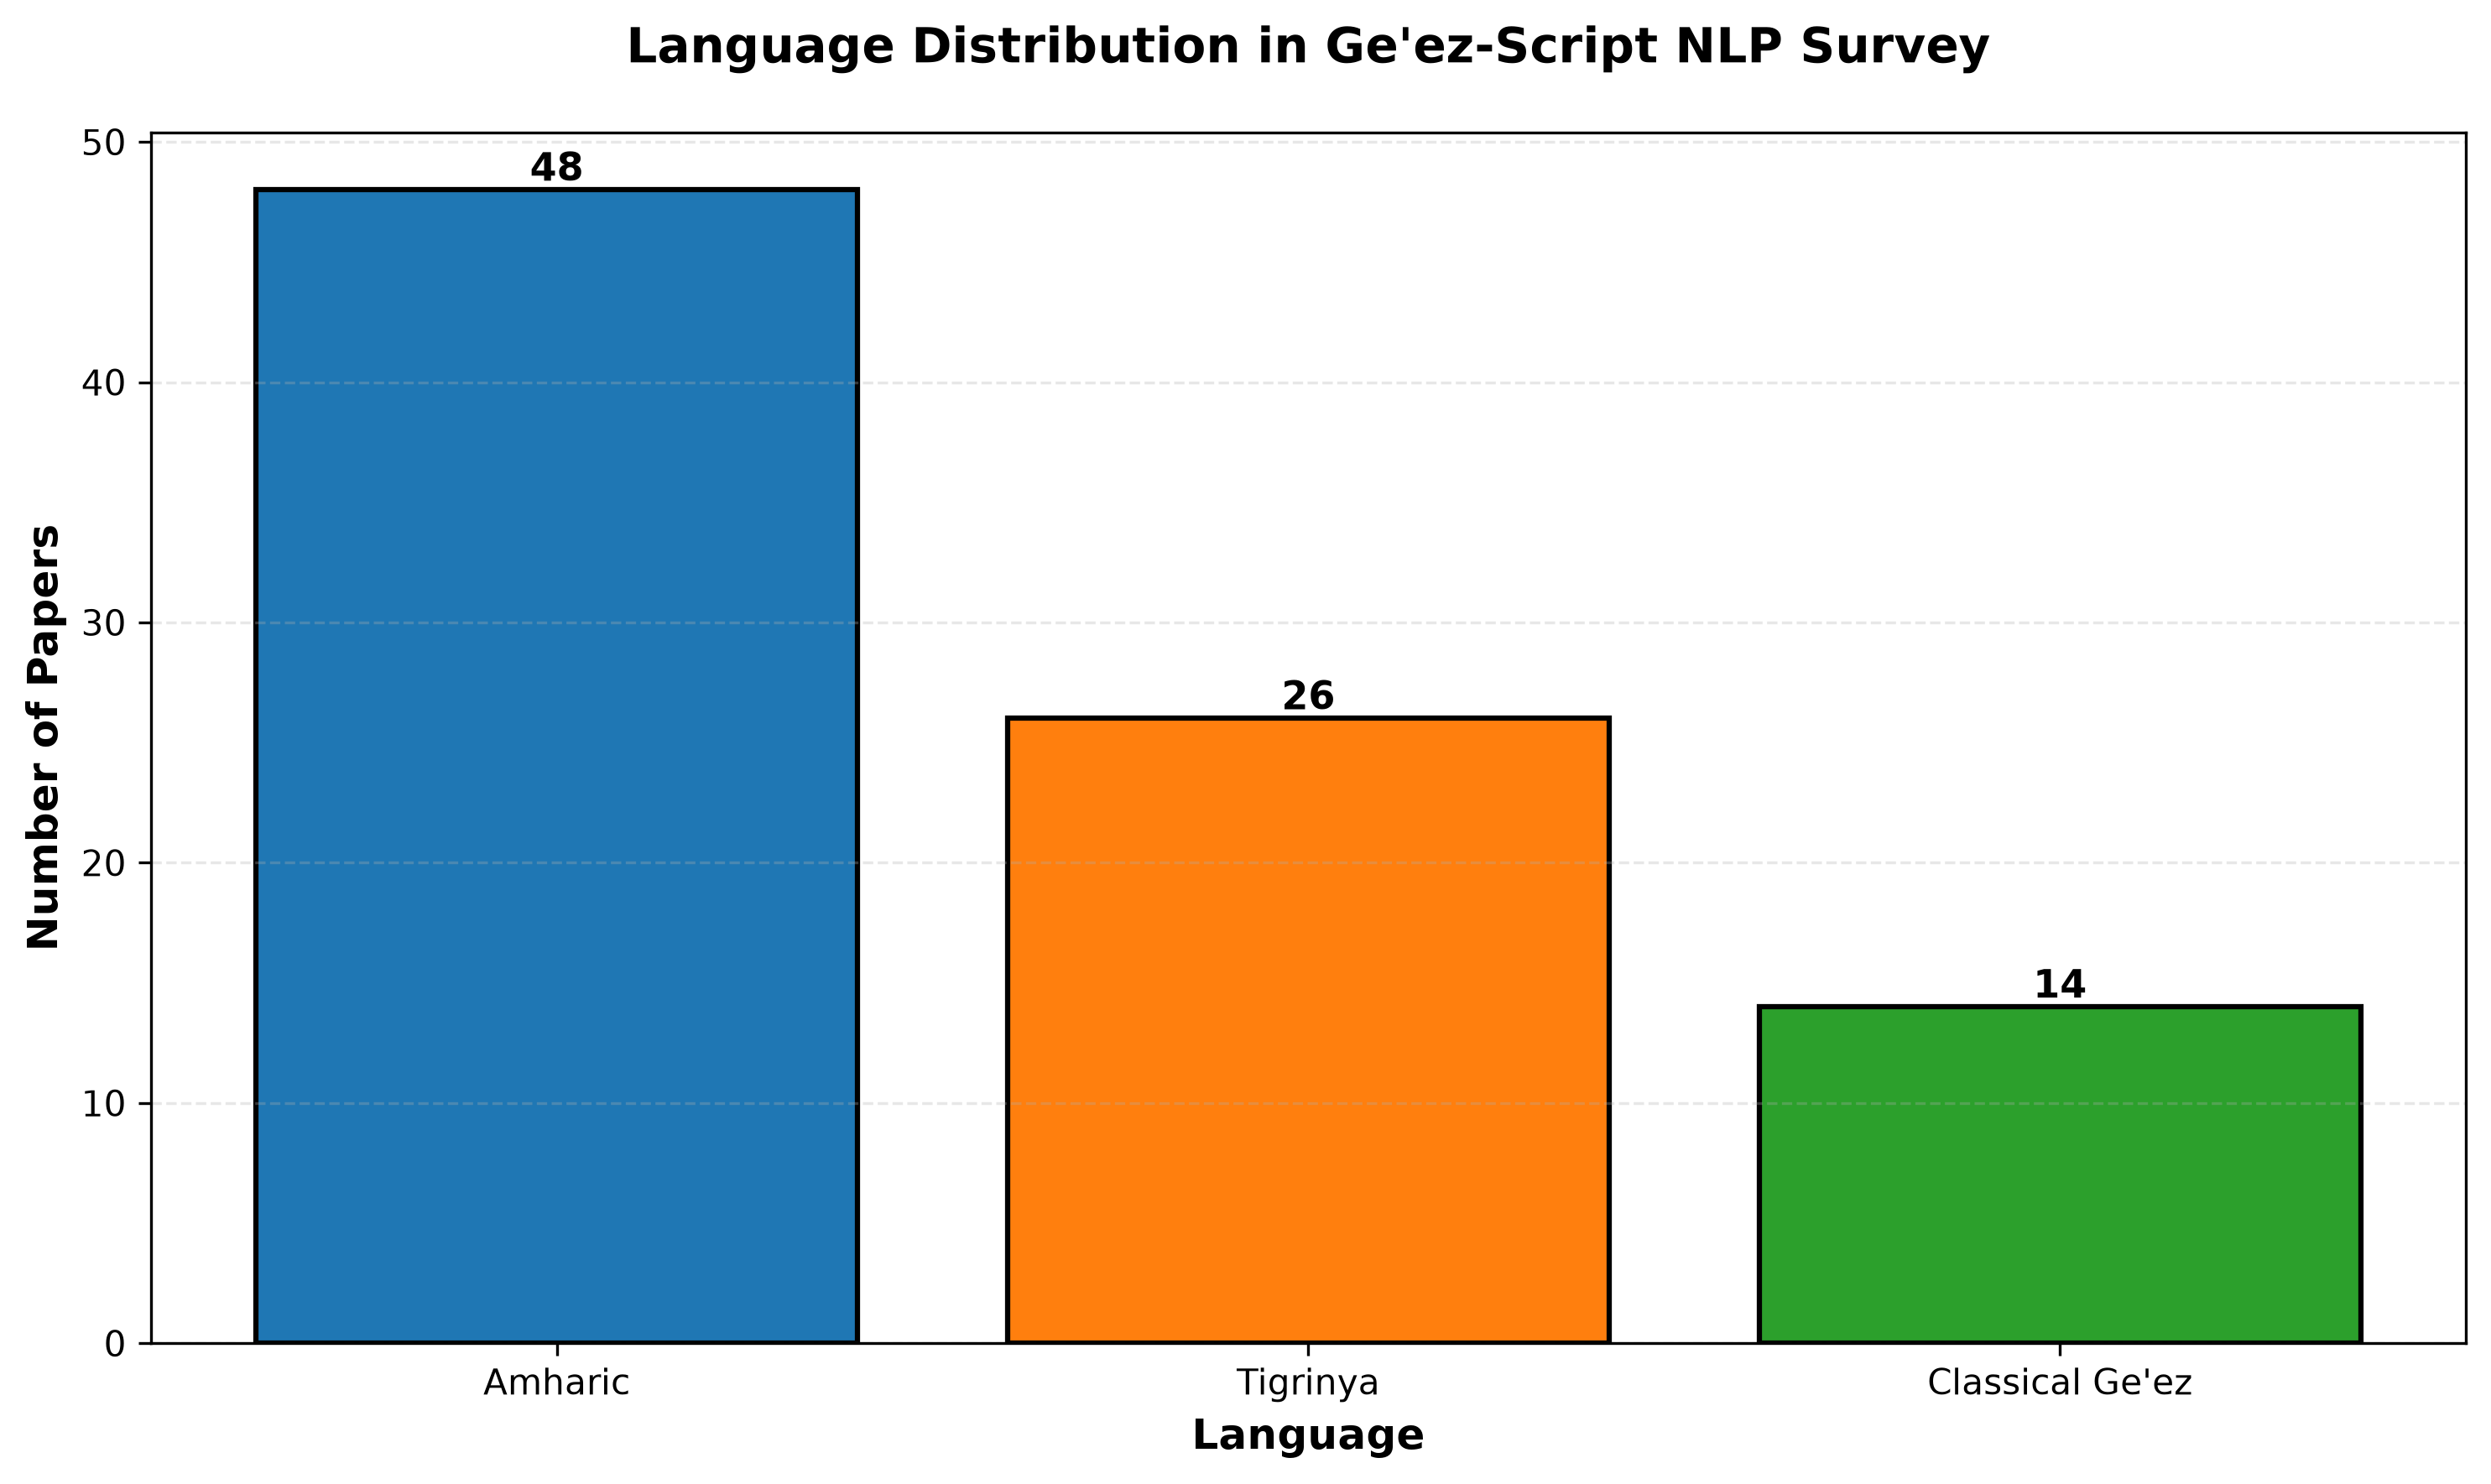
\includegraphics[width=0.8\textwidth]{chart_language_distribution.png}
\caption{Language distribution across the 69-paper verified literature corpus (overlapping count: a paper covering more than one Ge'ez-script language is counted under each). Amharic: 47 papers; Tigrinya: 26; Classical Ge'ez: 14.}\label{fig:language-dist}
\end{figure}

\begin{figure}[h]
\centering
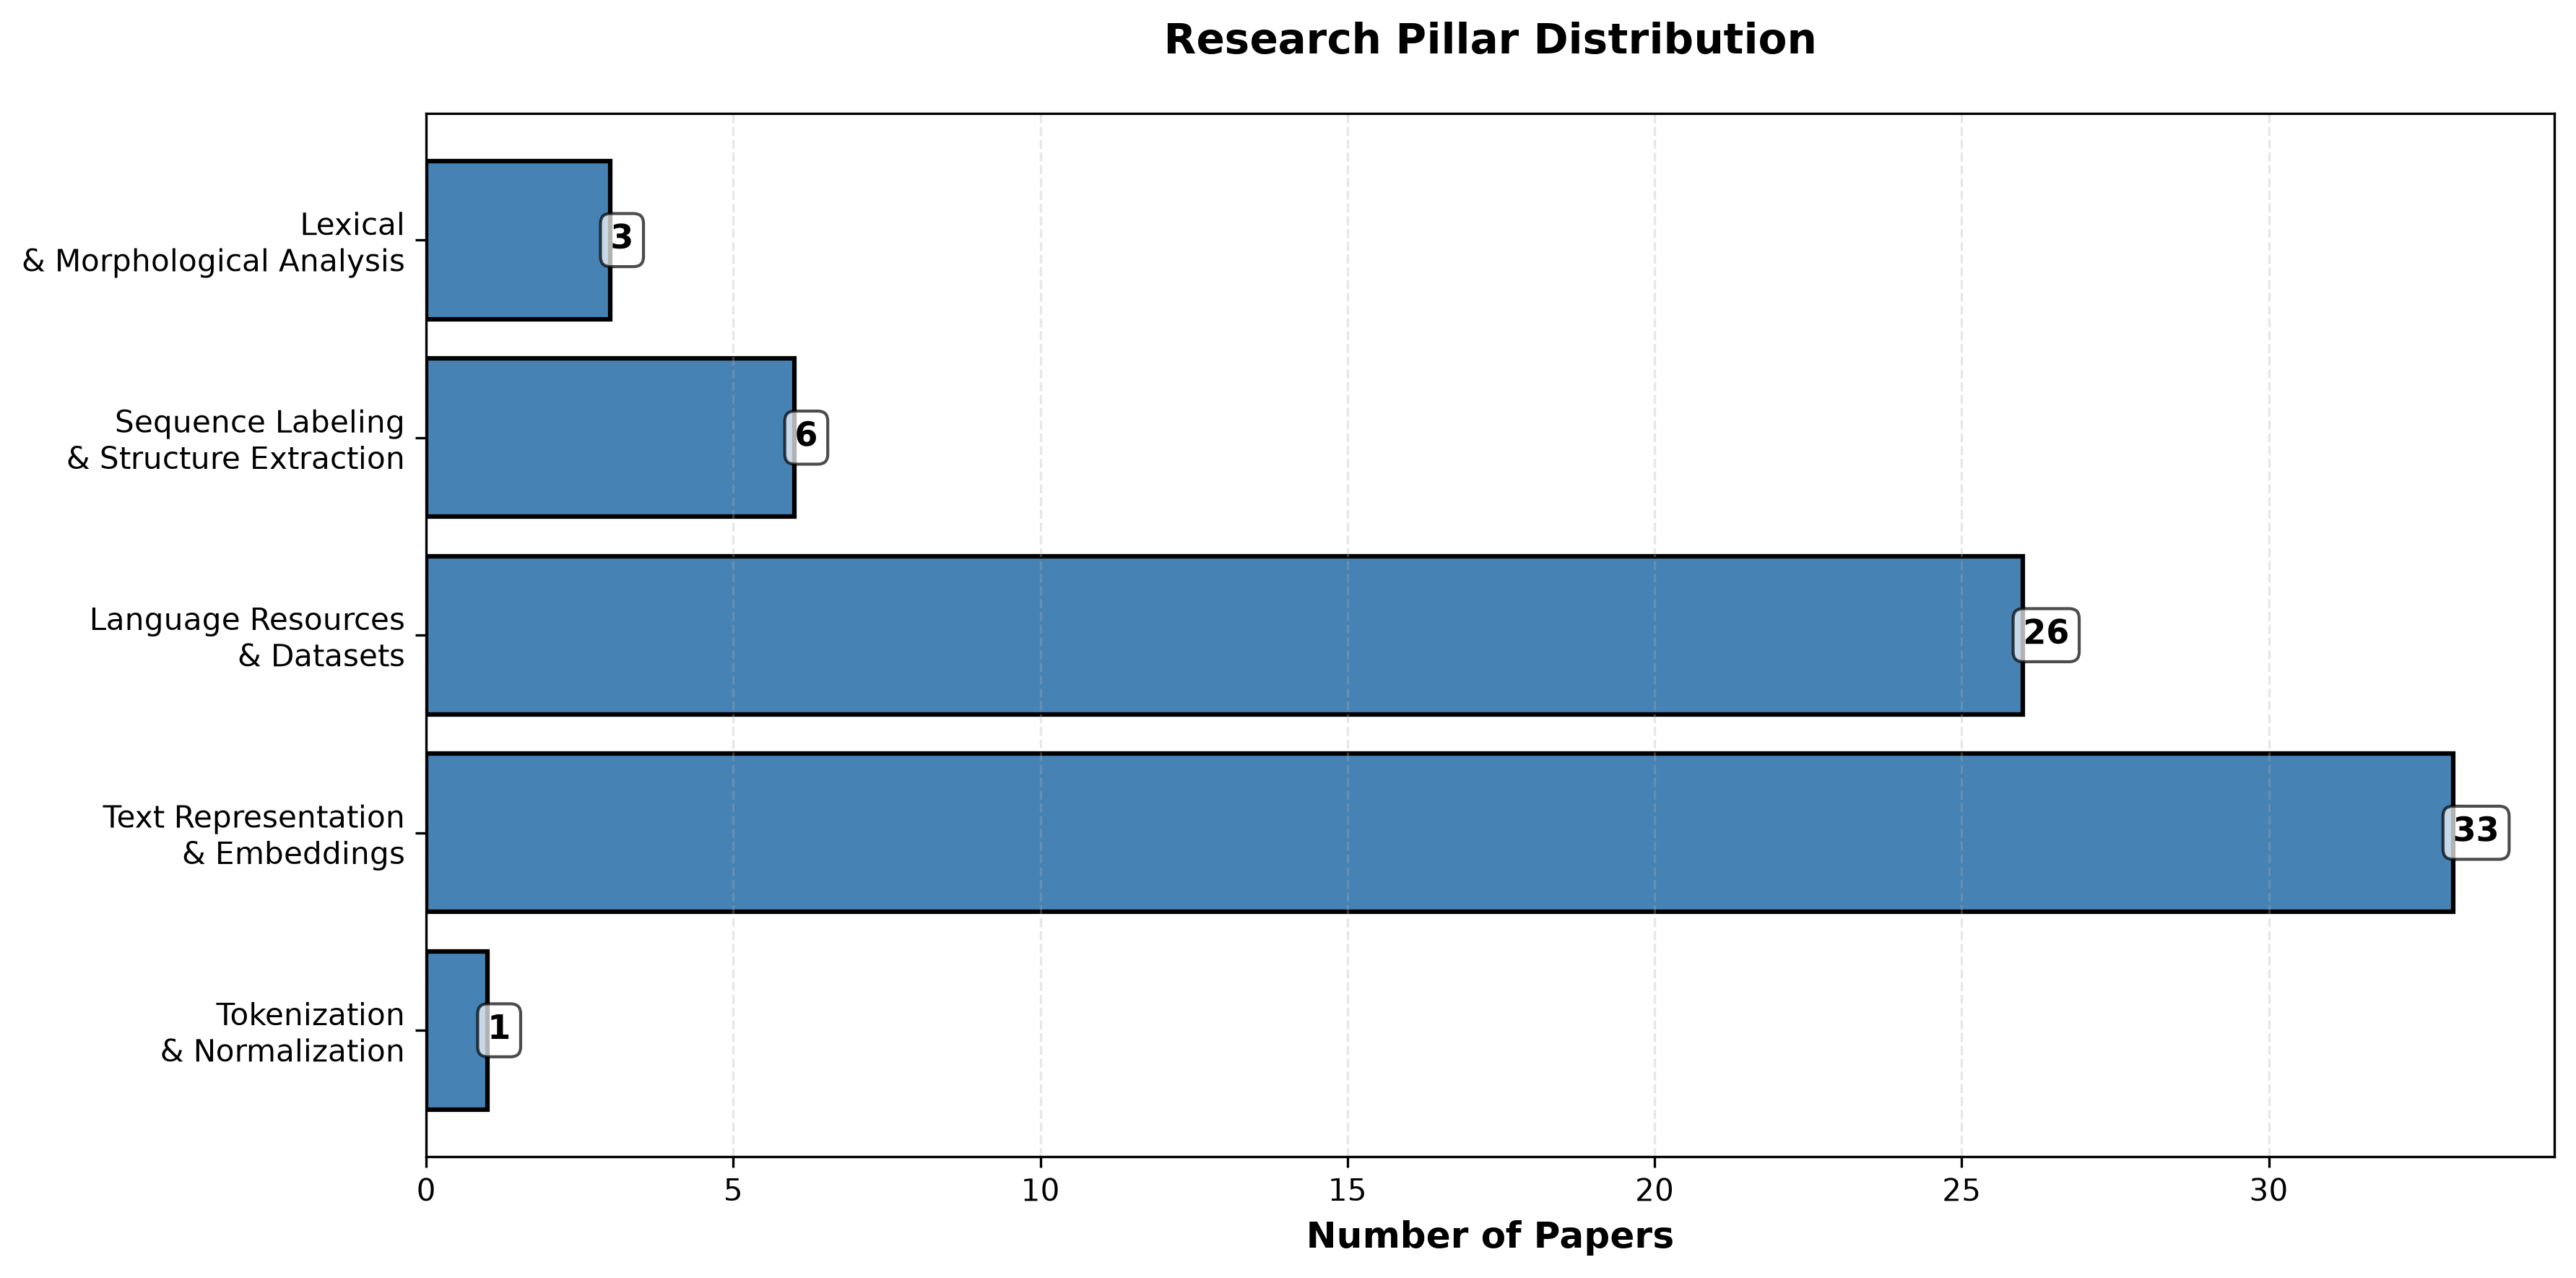
\includegraphics[width=0.8\textwidth]{chart_pillar_distribution.png}
\caption{Distribution of the 69-paper corpus across this project's canonical coding dimensions (Section~\ref{sec:literature-search}): Tokenisation \& Normalisation (1), Lexical \& Morphological Analysis (3), Text Representation \& Embeddings (33), Language Resources \& Datasets (26), Sequence Labeling \& Structure Extraction (6). These five categories map onto the manuscript's four-pillar framework (P1--P4) with Language Resources \& Datasets corresponding to the ``Other: Infrastructure'' category used elsewhere in this manuscript (Table~\ref{table:lit-by-pillar}).}\label{fig:pillar-dist}
\end{figure}

\begin{figure}[h]
\centering
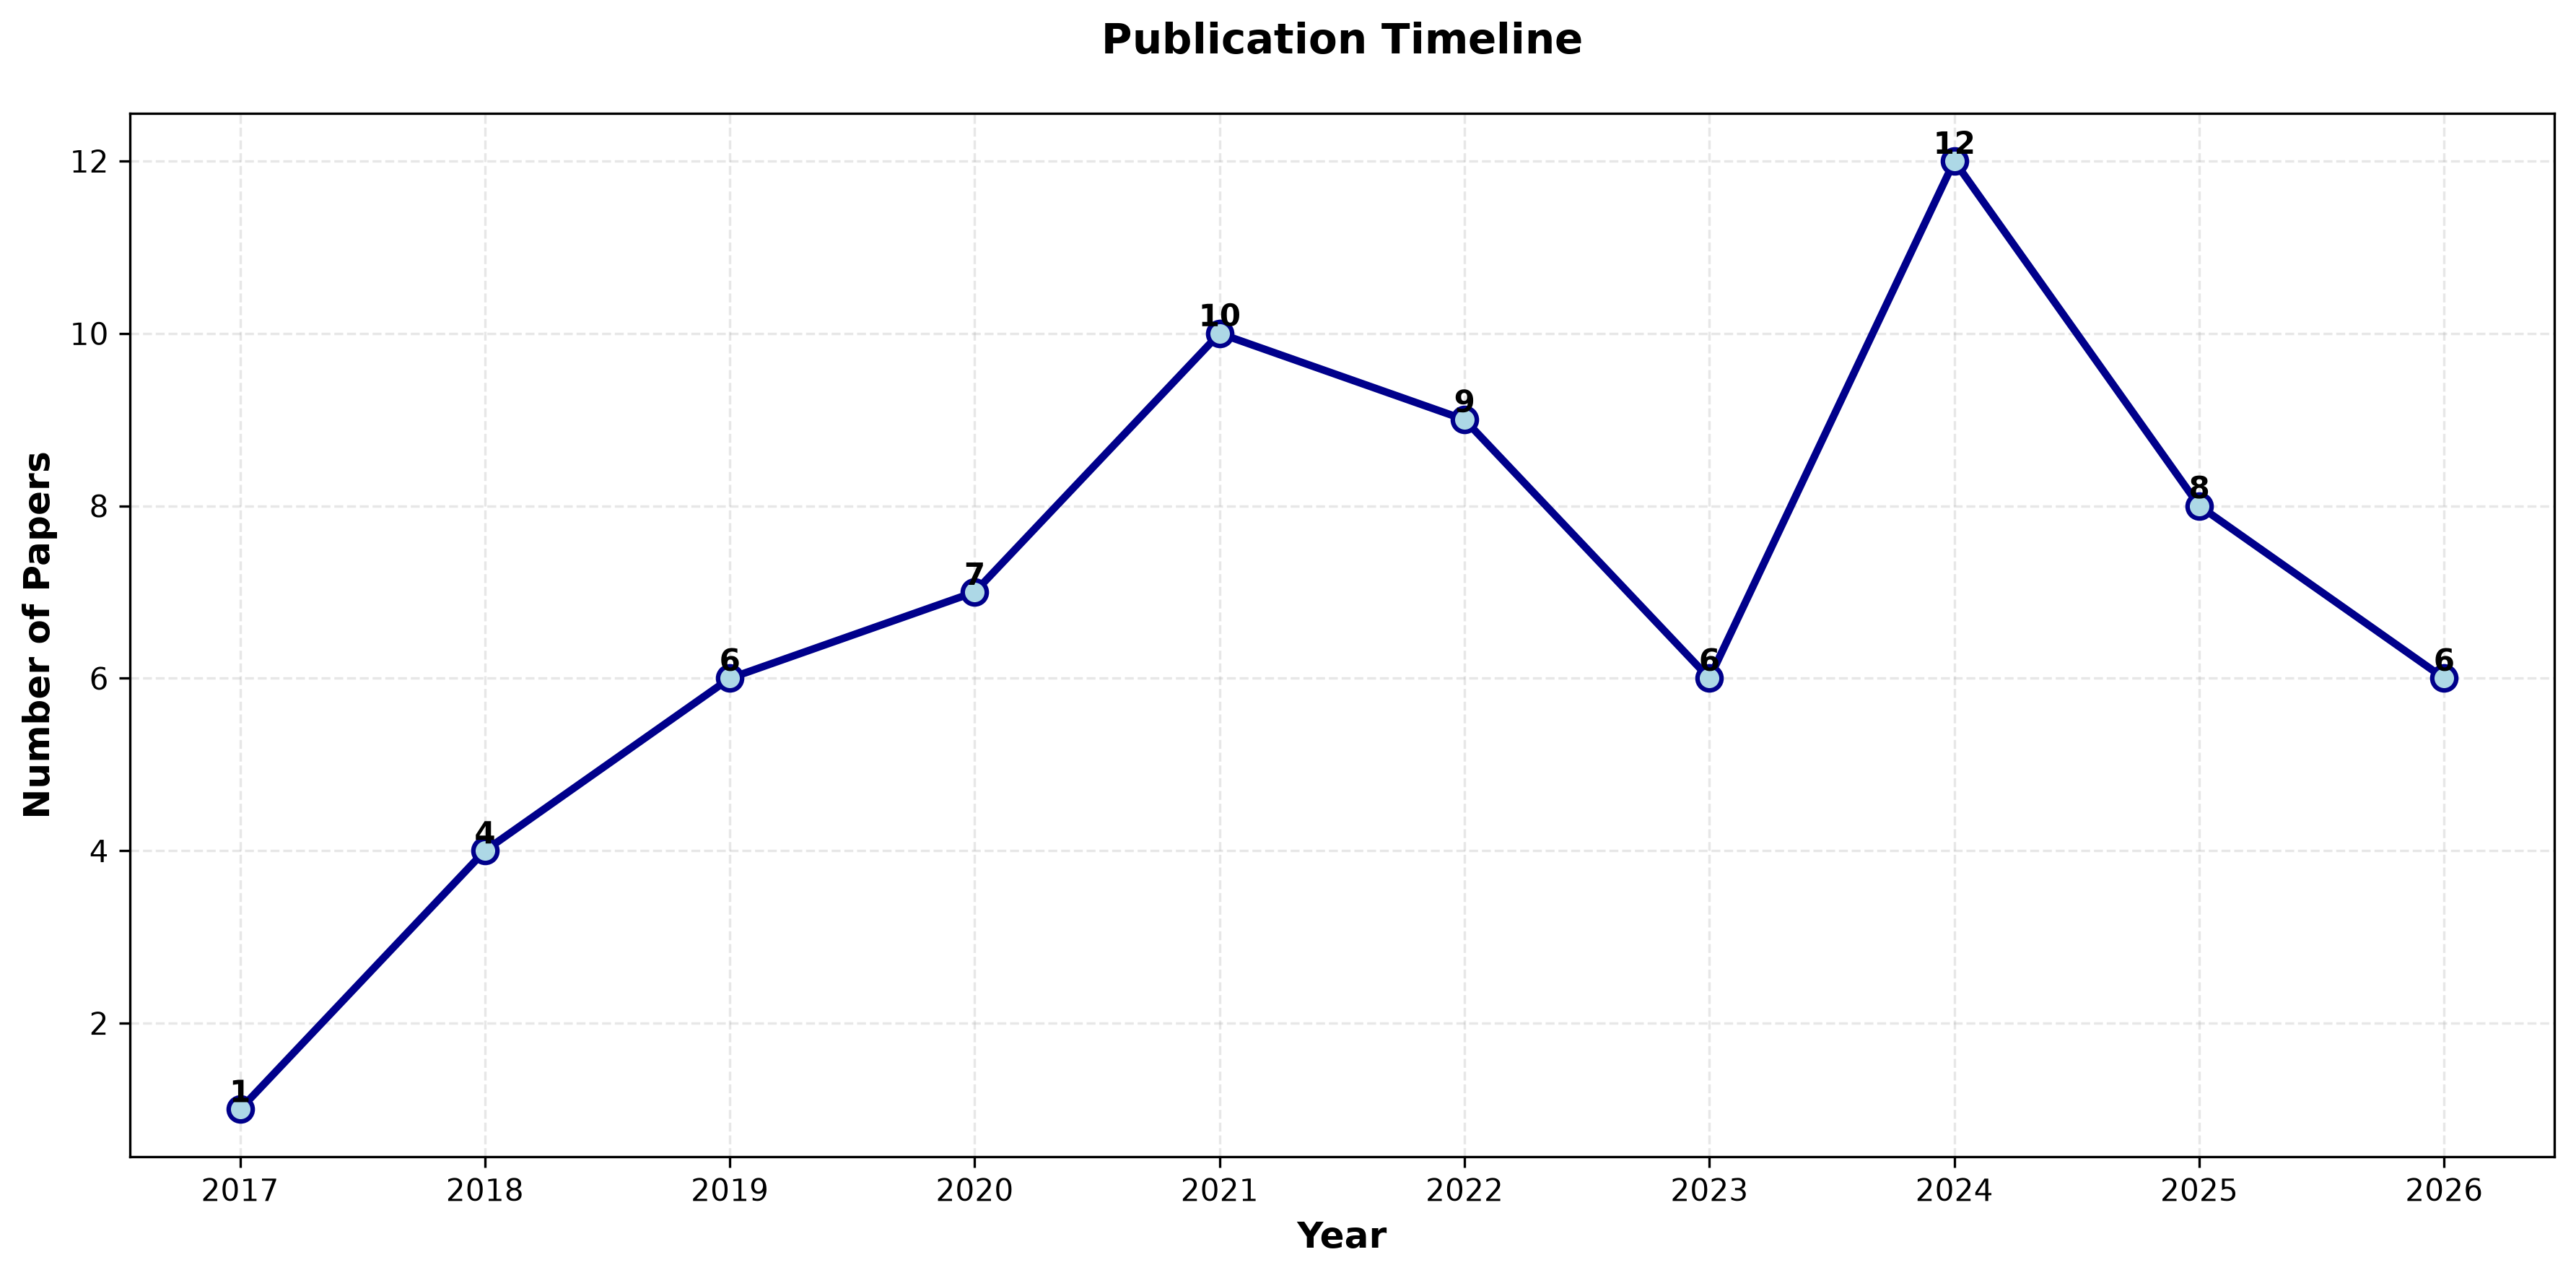
\includegraphics[width=0.8\textwidth]{chart_temporal_distribution.png}
\caption{Publication timeline of the 69-paper verified literature corpus, 2017--2026, tallied by exact publication year.}\label{fig:temporal-dist}
\end{figure}

\begin{figure}[h]
\centering
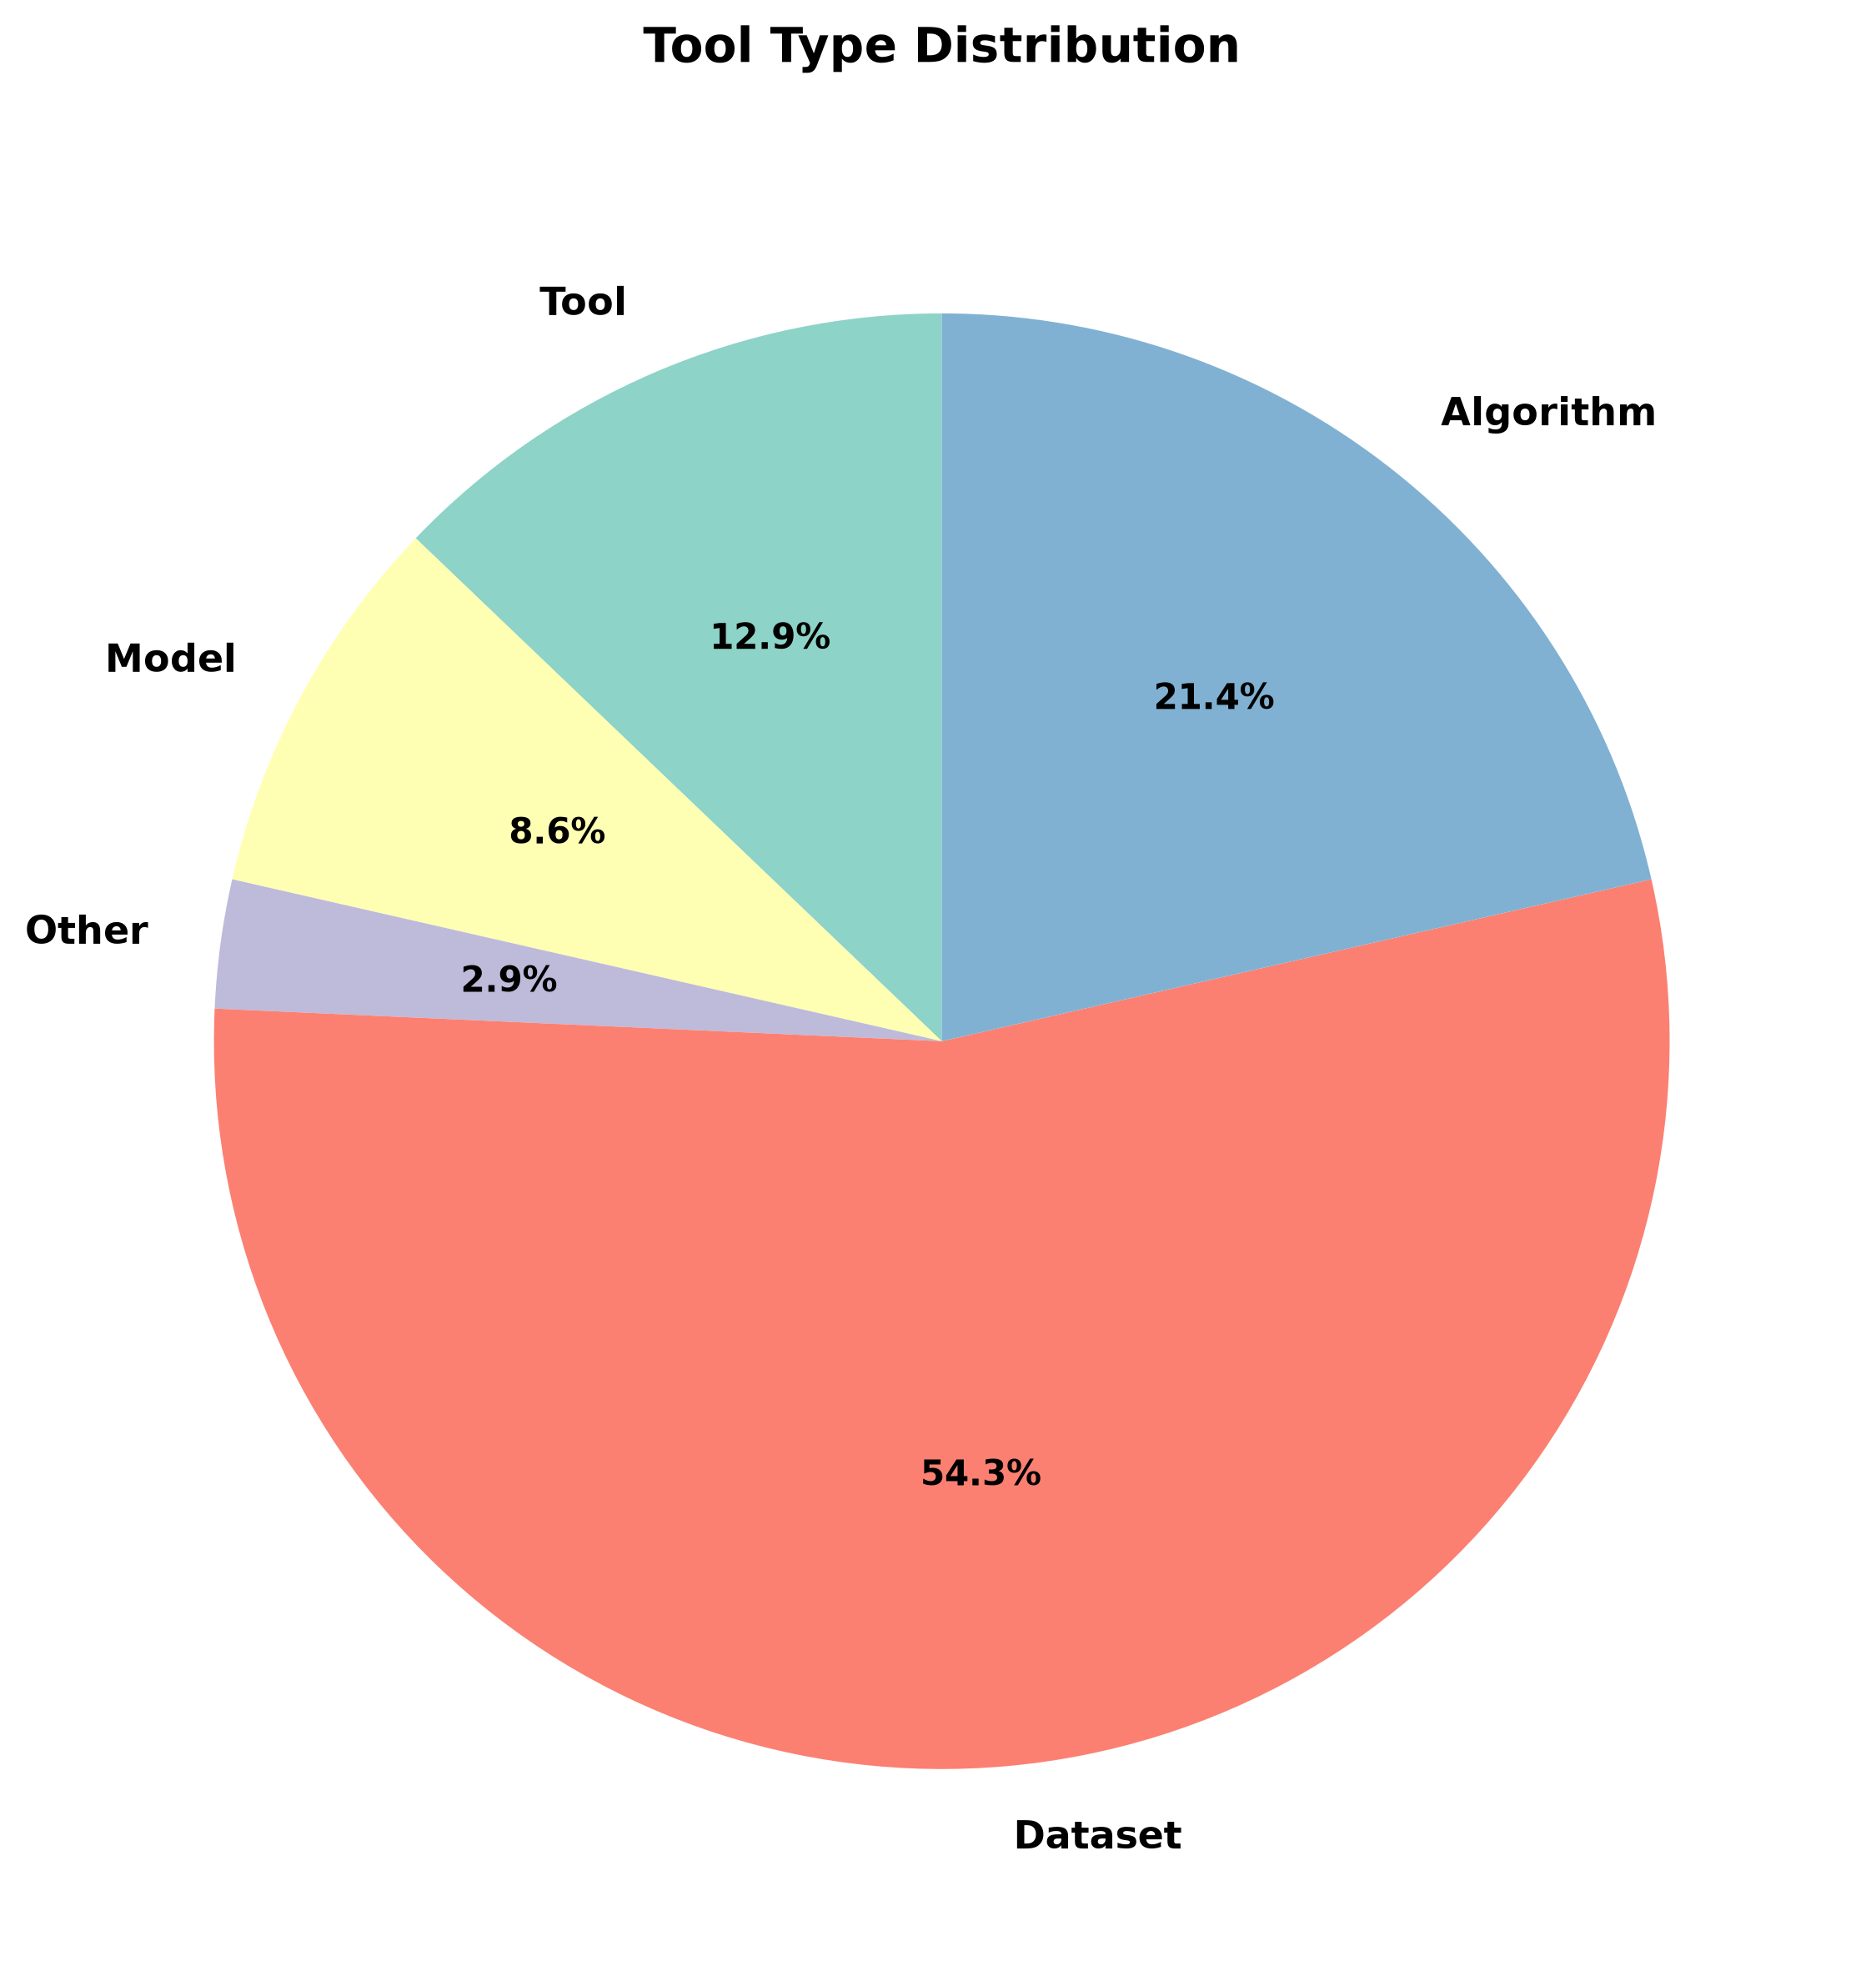
\includegraphics[width=0.7\textwidth]{chart_tool_type_distribution.png}
\caption{Distribution of the 69 corpus papers by primary contribution type (dataset, model, tool, algorithm, other). Each paper is assigned one type from its own \texttt{Datasets\_Count}, \texttt{Models\_Count} and \texttt{Tools\_Count} fields, in that order of precedence, falling back to its \texttt{Topics\_List}; papers with none of these artefacts are classed as algorithm papers (Section~\ref{sec:tools-from-corpus}). The unit is the paper, not the individual artefact, and papers are counted whether or not their artefacts have a confirmed public release (Table~\ref{table:tools-from-corpus}).}\label{fig:tool-type-dist}
\end{figure}

\section{Results}\label{sec:results}

\subsection{Tool Inventory}\label{sec:tool-inventory}

This survey reports one tool inventory, built and verified as described in Section~\ref{sec:tools-from-corpus}: \textbf{28 foundational NLP tools, models, datasets, and linguistic resources}, independently confirmed live on GitHub, Zenodo, PyPI, or HuggingFace at the time of writing (Table~\ref{table:tools-from-corpus}). Of these, 26 are individually traceable to a specific paper within the 69-paper literature corpus, and 2 (HornMorpho, MasakhaNER 1.0) are provenance-track additions whose originating papers fall outside the corpus (Section~\ref{sec:tool-discovery-scope-note}). Every tool, dataset, and model count in this section refers to Table~\ref{table:tools-from-corpus} and only to Table~\ref{table:tools-from-corpus}.

\begin{table}[h]
\caption{Distribution of the 28 verified tools across technical pillars (Table~\ref{table:tools-from-corpus}; 26 corpus-traceable plus two provenance-track additions, HornMorpho and MasakhaNER 1.0).}\label{table:overview}
\begin{tabular}{@{}lcc@{}}
\toprule
\textbf{Pillar} & \textbf{Count} & \textbf{\% of 28} \\
\midrule
P1: Tokenisation and Normalisation & 1 & 4\% \\
P2: Morphological Analysis and Synthesis & 1 & 4\% \\
P3: Embeddings, Language Models, and Evaluation & 16 & 57\% \\
P4: Sequence Labelling and Structure Extraction & 3 & 11\% \\
Other: Infrastructure & 7 & 25\% \\
\midrule
\textbf{Total} & \textbf{28} & \textbf{100\%} \\
\botrule
\end{tabular}
\end{table}

\subsection{Language Representation}\label{sec:language-representation}

Table~\ref{table:language} reports language coverage across the 28 verified tools using an overlapping accounting scheme: a tool supporting more than one Ge'ez-script language (e.g.\ GeezSwitch, EthioProverbEval, HornMorpho) is counted once under each language it supports, so the percentages sum to more than 100\%. Counts are tallied directly from the \textbf{Language(s)} column of Table~\ref{table:tools-from-corpus}.

\begin{table}[h]
\caption{Language coverage across the 28 verified tools (overlapping count; a tool supporting multiple languages is counted under each).}\label{table:language}
\begin{tabular}{@{}lcc@{}}
\toprule
\textbf{Language} & \textbf{Tools supporting it} & \textbf{\% of 28 tools} \\
\midrule
Amharic & 22 & 79\% \\
Tigrinya & 14 & 50\% \\
Classical Ge'ez & 6 & 21\% \\
\botrule
\end{tabular}
\end{table}

\noindent Amharic is the most represented language in this verified tool set, followed by Tigrinya; Classical Ge'ez is the least represented of the three at the tool level, consistent with its status as the least-represented language in the literature corpus itself (Table~\ref{table:lit-by-language}). No tool in Table~\ref{table:tools-from-corpus} is dedicated to Classical Ge'ez alone: all six tools that support Ge'ez also cover both Amharic and Tigrinya.

\subsection{Technical Pillar Analysis}\label{sec:pillars}

P3 (embeddings, language models, and evaluation) is the largest pillar in the verified tool set (16 of 28 tools, 57\%), reflecting the broader trend toward pre-trained language models and dense-retrieval methods in this literature. Other/Infrastructure resources (datasets, corpora) account for a further 7 tools (25\%). P4 (sequence labelling) is represented by 3 tools, one of which (MasakhaNER 1.0) is a provenance-track addition rather than a corpus paper's own contribution (Section~\ref{sec:tool-discovery-scope-note}). P1 (tokenisation and normalisation) is represented by a single verified tool, amseg (P013). \textbf{No P2 (morphological analysis and synthesis) tool from the 69-paper corpus itself has an independently confirmed public repository}: morphology-focused artefacts described in the reviewed papers (e.g.\ the Ge'ez Synthesizer, P042~\citep{gidey_morphological_2024}; the Tigrigna verb morphological analyzer, P072~\citep{gebremeskel_tigrigna_2023}; the Amharic morphology generator, P070~\citep{nigusie_suffixinflectional_2024}) exist and are named in their source papers, but no live GitHub, Zenodo, PyPI, or HuggingFace link for any of them could be independently confirmed, so none is counted in this corpus-derived pillar breakdown. This is reported as an evidence gap in tool-repository discoverability among corpus papers specifically, not as evidence that no P2 tool exists in the wider field: HornMorpho, a public, actively maintained morphological analyser/generator whose Amharic and Tigrinya components fall within this survey's scope (its Oromo component is Latin-script and out of scope, Section~\ref{sec:tools-from-corpus}), is added to Table~\ref{table:tools-from-corpus} under the provenance-track standard of Section~\ref{sec:dual-standard}, giving 1 verified P2 tool overall (Table~\ref{table:overview}) even though none of the three P2-relevant corpus papers has its own confirmable release.

\subsection{Sequence Labelling: Verified vs.\ Described Artefacts}\label{sec:p4}

Three P4 tools in Table~\ref{table:tools-from-corpus} have an independently confirmed public repository: the Amharic UD Treebank (P017) and the Tigrinya NER dataset associated with P015, both corpus-traceable, plus MasakhaNER 1.0, a provenance-track addition covering Amharic (Section~\ref{sec:tool-discovery-scope-note}). An earlier candidate, MasakhaPOS, was removed after verification against its own paper showed it does not cover any Ge'ez-script language (Section~\ref{sec:tool-discovery-scope-note}). Beyond these, the 69-paper corpus describes further sequence-labelling artefacts -- including TiNC24 (P075~\citep{berhane_towards_2025}), ANEC (P028~\citep{jibril_anec_2022}), and EthioMT-adjacent resources -- for which no independently confirmable public repository link exists. These are named and cited in their respective papers (Section~\ref{sec:tools-from-corpus}) but are not counted among the verified tools, since this survey counts only artefacts with an independently confirmable public release.

\section{Research Asymmetry}\label{sec:asymmetry}

Based on the literature corpus (Table~\ref{table:lit-by-language}) and the tool inventory (Table~\ref{table:language}), Amharic is the most represented Ge'ez-script language in both the literature (68\% of 69 papers) and the tool inventory (79\% of 28 tools); Tigrinya is second in both (38\% of papers; 50\% of tools); Classical Ge'ez is the least represented in both (20\% of papers; 21\% of tools) -- a consistent, non-trivial gap favouring Amharic across both measures. Eight tools in the verified inventory (Table~\ref{table:tools-from-corpus}) cover more than one of the three languages: EthioPOS, the EthioLLM model family, GeezSwitch, GeezSwitch-data, EthioProverbEval and the ProverbEval benchmark cover all three, and EthioEmo-intensities and HornMorpho cover Amharic and Tigrinya. Most of these are multilingual resources for Ethiopian languages in general (several also cover Oromo, Somali, or English), and only GeezSwitch and GeezSwitch-data are designed around the Ge'ez script itself. None is a script-level transfer-learning framework spanning all three languages, and they follow no shared annotation or evaluation conventions.

LGSE (P002~\citep{teklehaymanot_lgse_2026}) and MoVoC (P001~\citep{teklehaymanot_movoc_2025}) are two independently-verified papers in the corpus (Section~\ref{sec:literature-search}) whose stated contributions include cross-lingual or cross-script components for Amharic, Tigrinya, and/or Classical Ge'ez jointly; neither had an independently confirmable, live public repository of \emph{the specific artefact each paper reports} at the verification date (Section~\ref{sec:tool-discovery}), and so neither is counted among the verified tools in Table~\ref{table:tools-from-corpus}, despite both papers being part of the verified literature corpus. A release matching MoVoC's corrected version (ACL Anthology revision~2, 21 October 2026) has since appeared and is recorded in the repository's inventory addenda.

\section{Survey Limitations}\label{sec:limitations}

We acknowledge several limitations:

\begin{enumerate}
    \item \textbf{Publication bias:} Focus on peer-reviewed papers may undercount community contributions.
    \item \textbf{Venue bias:} Concentration on major conferences may miss specialised venues.
    \item \textbf{Language bias:} English-only publication requirement may exclude relevant work.
    \item \textbf{Reproducibility:} Many tools lack maintained documentation or open-source code.
    \item \textbf{Temporal bias:} 2016--2026 window omits earlier work and cannot predict trends.
    \item \textbf{Tool discovery bias:} Published tools overrepresented relative to unpublished community work.
    \item \textbf{Completeness:} Some tools may not have been discovered despite systematic search; a described artefact whose public repository could not be independently confirmed is excluded from the verified tool count entirely, even if the paper itself asserts a public release (Section~\ref{sec:pillars}).
    \item \textbf{Known omissions:} Some in-scope work was not captured by the search, including Tigrinya part-of-speech tagging on the Nagaoka Tigrinya Corpus \citep{tedla_tigrinya_2016}, LSTM-based Tigrinya morphological segmentation \citep{tedla_morphological_2018}, and deep-learning part-of-speech tagging for Tigrinya and Tigre \citep{kapociute_northern_2020}. These fall in Pillars 2 and 4; adding them would not change the ordering of the pillars, in which P1 and P2 remain the least represented (1 and 3 of 69 papers).
    \item \textbf{No inter-rater agreement statistic:} All extracted data and category assignments (language, pillar, artefact type) were independently reviewed by all co-authors, and disagreements were resolved by discussion. Formal double-coding with an inter-rater agreement statistic was not performed.
    \item \textbf{PRISMA intermediate-stage counts unavailable:} No preserved search log exists for the Identification or Screening stages, so Figure~\ref{fig:prisma-flow} reports process descriptions rather than invented counts for those stages; only the full-text assessment (71 records, 2 excluded) and the final included-studies count ($n=69$) are independently verifiable (Section~\ref{sec:prisma}).
    \item \textbf{P2 verification gap:} No morphology-and-synthesis (P2) tool from the 69-paper corpus has an independently confirmed public repository at the verification date (Section~\ref{sec:pillars}); this is reported as a discoverability gap, not as an absence of such work.
    \item \textbf{No independent data-quality assessment:} This survey verifies that a paper, tool, or dataset \emph{exists} and matches its own reported provenance (Section~\ref{sec:dual-standard}); it does not independently assess the annotation quality, inter-annotator agreement, label correctness, or cleanliness of any dataset it catalogues. Inclusion in this survey's corpus or tool inventory reflects peer-review status or public-repository existence, neither of which is equivalent to a quality audit of the underlying data. A dataset's fitness for a specific downstream use should be assessed against its own source paper's reported methodology, not inferred from its presence here.
\end{enumerate}

\section{Research Priorities}\label{sec:agenda}

The following seven priorities follow directly from the gaps quantified in Sections~\ref{sec:results}--\ref{sec:asymmetry}, with the final two priorities addressing, respectively, a methodological limitation of this survey itself (Section~\ref{sec:limitations}) and a scope boundary of its own literature search (Section~\ref{sec:literature-search}), rather than corpus-derived quantitative gaps.

\subsection{Priority 1: Shared Tokenisation Across the Three Languages}

\textbf{Evidence:} Table~\ref{table:overview} shows only 1 of 28 verified tools (4\%) addresses P1 (tokenisation and normalisation); Table~\ref{table:lit-by-pillar} shows the same pattern in the literature (1 of 69 papers, 1\%). That one tool, amseg (P013), is Amharic-only: no verified P1 tool in this survey covers more than one Ge'ez-script language. The gap this priority addresses is accordingly total, not partial.

\textbf{Priority:} A tokeniser evaluated across Amharic, Tigrinya, and Classical Ge'ez jointly, with a publicly documented release, would address the near-absence of P1 tools identified above.

\subsection{Priority 2: Morphological Analysis with a Verifiable Public Release}

\textbf{Evidence:} No P2 (morphological analysis and synthesis) tool from a corpus paper itself has a confirmed public repository (Table~\ref{table:overview}; Section~\ref{sec:pillars}), although three P2-relevant papers exist in the corpus (P042, P070, P072) without an independently confirmable release of their own. HornMorpho, a pre-2016 tool whose Amharic and Tigrinya components are in scope (its Oromo component is Latin-script, Section~\ref{sec:tools-from-corpus}), fills this pillar under the provenance-track standard (Section~\ref{sec:dual-standard}) but is not a contribution of any paper in this survey's corpus.

\textbf{Priority:} Publishing a morphological analyser or synthesiser \emph{from a corpus-eligible paper} for any of the three languages with a stable, versioned public identifier (Section~\ref{sec:dual-standard}) would close this specific verification gap; separately, coordinating with or extending an existing tool such as HornMorpho, rather than duplicating it, would make more efficient use of already-available infrastructure.

\subsection{Priority 3: Continued Investment in P3 Balanced Against Other Pillars}

\textbf{Evidence:} P3 (embeddings, language models, and evaluation) accounts for 16 of 28 verified tools (57\%) and 33 of 69 papers (48\%), the largest share of both the tool inventory and the literature (Tables~\ref{table:overview}, \ref{table:lit-by-pillar}).

\textbf{Priority:} Given the concentration of activity in P3, future work targeting P1, P2, or P4 would address pillars that are comparatively underserved rather than add to the pillar already best represented.

\subsection{Priority 4: Verifiable Releases for Sequence-Labelling Resources}

\textbf{Evidence:} Only 2 of 69 papers with a P4 contribution have an independently confirmed public repository from within the corpus itself (the Amharic UD Treebank, P017, and the Tigrinya NER dataset, P015; Section~\ref{sec:p4}); a third verified P4 tool, MasakhaNER 1.0, is a provenance-track addition from outside the corpus (Section~\ref{sec:tool-discovery-scope-note}). Further P4 artefacts (e.g.\ TiNC24, ANEC) are described in the literature but have no confirmable public release at the time of writing.

\textbf{Priority:} Publishing the P4 artefacts already described in the literature under a stable public identifier would increase the corpus-traceable verified P4 count without requiring new research.

\subsection{Priority 5: Cross-Language Coordination}

\textbf{Evidence:} Eight of the 28 verified tools cover more than one of the three languages, six of them all three (Section~\ref{sec:asymmetry}), but none functions as a shared framework across the three, and each follows its own annotation and evaluation conventions.

\textbf{Priority:} Coordinating existing single-language efforts under shared annotation and evaluation conventions would let future tools reuse resources across Amharic, Tigrinya, and Classical Ge'ez rather than duplicate work already done for one language.

\subsection{Priority 6: Independent Data-Quality Assessment}

\textbf{Evidence:} This survey verifies that a dataset or tool exists and matches its own reported provenance (Section~\ref{sec:dual-standard}); it does not independently assess annotation quality, inter-annotator agreement, label correctness, or corpus cleanliness for any entry in the literature corpus or tool inventory (Section~\ref{sec:limitations}). Inclusion here reflects peer-review status or public-repository existence, neither of which is a substitute for a quality audit of the underlying data.

\textbf{Priority:} Before any dataset catalogued in this survey is adopted as a foundation for further work, its annotation methodology and reported quality metrics (where available) should be independently reviewed rather than assumed from its inclusion here; where a dataset's source paper does not report inter-annotator agreement or an equivalent quality measure, generating one would materially increase confidence in downstream use. A follow-up systematic quality audit of the tool inventory -- assessing annotation methodology, agreement statistics, and known corpus issues per entry -- would substantially strengthen the evidentiary basis this survey's tool-centred approach establishes.

\subsection{Priority 7: Reuse of Classical Semitic Studies and Digital Humanities Resources}

\textbf{Evidence:} This survey's literature search (Section~\ref{sec:literature-search}) is deliberately scoped to NLP venues and NLP-adjacent provenance-track sources; it does not survey classical Semitic studies, philology, or digital-humanities venues. Long-running projects in those fields, sustained by independent research funding (including European Research Council and national research-council grants), have produced extensive manuscript digitisations, digital editions, Unicode transcriptions of Ge'ez texts, workflows for TEI annotation, manuals for linguistic tagging, guidelines for OHR/OCR processing, and parsing applications built for research and teaching. These resources have rarely been carried across into working digital tools for the language communities that use the Ge'ez script today. A contributing factor is that much of the material was, at various points, processed via transliteration into extended Latin script, and so was not originally tailored for reuse within the original writing system. One concrete example, verified directly for this survey: Liuzzo's Ge'ez Morphological Parser Application \citep{liuzzo_geez_2019}, developed under the ERC-funded TraCES project, has a stable, citable public identifier (DOI: 10.25592/uhhfdm.125) but is no longer operating in its original form; it is currently being redeveloped on GitHub (\texttt{MaSNaqtu/geez-parser}) under the Swiss National Science Foundation-funded MiTAnIm project. Because this survey's search was scoped to NLP venues by design (Section~\ref{sec:literature-search}), resources of this kind are structurally invisible to it despite being directly relevant to Ge'ez-script computational work; they are named here as a known category of out-of-frame resources, not because this survey systematically searched for them.

\textbf{Priority:} Ge'ez-script NLP across all four methodological pillars and the Other/Infrastructure category (Section~\ref{sec:pillars}) could be advanced substantially through deliberate collaboration with classical Semitic studies and digital-humanities projects, specifically to reuse and further develop the datasets, annotated corpora, and parsing tools those projects have already produced. The task is less one of building from scratch than of strategic recycling and up-cycling: adapting material that exists but is oriented towards philological research rather than language technology, and in particular converting transliterated Latin-script resources back into the Ge'ez script in which the language communities actually read and write. Treated this way, work already funded and completed in adjacent fields becomes directly usable for Ge'ez-script NLP, avoiding duplication of effort in a setting where resources are scarce. For a broader overview of ongoing and completed projects in this space (e.g.\ Ethio-SPaRe, TraCES, Beta Masaheft), see the survey article by the Digital Orientalist \citep{digitalorientalist2026}.

\section{Conclusion}\label{sec:conclusion}

This survey documents a 28-tool inventory of foundational tools, models, datasets, and linguistic resources independently confirmed publicly available on GitHub, Zenodo, PyPI, or HuggingFace, distributed across four technical pillars (P1: 1 tool, 4\%; P2: 1 tool, 4\%; P3: 16 tools, 57\%; P4: 3 tools, 11\%; Other: Infrastructure: 7 tools, 25\%), alongside a PRISMA 2020-guided review of 69 individually live-verified publications (Section~\ref{sec:prisma}). Of the 28 tools, 26 are individually traceable to a specific paper in the 69-paper literature corpus; two (HornMorpho, MasakhaNER 1.0) are provenance-track additions whose originating papers fall outside the corpus (Section~\ref{sec:tool-discovery-scope-note}). Amharic is the most represented language in both the literature (68\% of papers) and the tool inventory (79\% of tools), Tigrinya is second in both (38\%; 50\%), and Classical Ge'ez is the least represented in both (20\%; 21\%). No P2 (morphological analysis and synthesis) tool from the reviewed papers themselves has an independently confirmed public repository; the survey's single verified P2 tool, HornMorpho, is a provenance-track addition from outside the corpus, not evidence that any corpus paper's own morphological tool is publicly available. P1 (tokenisation and normalisation) is limited to a single verified tool, amseg, which is Amharic-only; no corpus paper's own tokeniser with a confirmed public release covers more than one Ge'ez-script language. Sequence-labelling (P4) infrastructure is limited to 3 verified tools, one of which (MasakhaNER 1.0) is likewise a provenance-track addition; further artefacts of both kinds are described in the literature but lack an independently confirmable public release. Eight tools cover more than one of the three languages, but none is a script-level transfer framework, and they share no common annotation or evaluation standard.

The seven priorities in Section~\ref{sec:agenda} follow directly from the gaps identified above: the absence of a confirmed P2 repository, the concentration of tool development in P3, the lack of coordination across the three languages sharing the Ge'ez script, and -- distinct from these corpus-derived gaps -- this survey's own lack of independent data-quality assessment for any catalogued dataset or tool, and its literature search's exclusion, by design, of classical Semitic studies and digital-humanities resources directly relevant to Ge'ez-script computational work.

\backmatter

\bmhead{Acknowledgements}

This systematic review was conducted as part of ongoing research into low-resource language technology at the L3S Research Center, Leibniz University Hannover. We thank the Ge'ez-script NLP community, particularly all contributors to this paper.
\begin{appendices}

\section{Complete List of the 69-Paper Verified Literature Corpus}\label{app:corpus-list}

Table~\ref{table:corpus-full-list} lists every paper in the verified literature corpus (Section~\ref{sec:literature-search}) with its citation key, providing a full, individually citable record of the systematic review's included studies.

\begin{longtable}{@{}p{1.1cm}p{8.5cm}p{2.3cm}@{}}
\caption{Complete list of the 69 papers in the verified literature corpus, with citation keys. Full bibliographic details appear in the References section.}\label{table:corpus-full-list} \\
\toprule
\textbf{ID} & \textbf{Title} & \textbf{Citation} \\
\midrule
\endfirsthead
\multicolumn{3}{@{}l}{\textit{Table~\ref{table:corpus-full-list} continued from previous page}} \\
\toprule
\textbf{ID} & \textbf{Title} & \textbf{Citation} \\
\midrule
\endhead
\midrule
\multicolumn{3}{r@{}}{\textit{continued on next page}} \\
\endfoot
\bottomrule
\endlastfoot
P001 & MoVoC: Morphology-Aware Subword Construction for Ge'ez Script Languages & \citep{teklehaymanot_movoc_2025} \\
P002 & LGSE: Lexically Grounded Subword Embedding Initialization for Low-Resource Language Adaptation & \citep{teklehaymanot_lgse_2026} \\
P003 & Optimized Text Embedding Models and Benchmarks for Amharic Passage Retrieval & \citep{mekonnen_optimized_2025} \\
P004 & Natural Language Processing for Tigrinya: Current State and Future Directions & \citep{gaim_tigrinya_2025} \\
P005 & Natural Language Processing in Ethiopian Languages: Current State, Challenges, and Opportunities & \citep{tonja_natural_2023} \\
P006 & EthioLLM: Multilingual Large Language Models for Ethiopian Languages with Task Evaluation & \citep{tonja_ethiollm_2024} \\
P007 & Machine Translation for Ge'ez Language & \citep{wassie_machine_2023} \\
P009 & Supervised Machine Learning based Amharic Text Complexity Classification Using Automatic Annotator Tool & \citep{nigusie_supervised_2025} \\
P011 & Exploring Amharic Sentiment Analysis from Social Media Texts: Building Annotation Tools and Classification Models & \citep{yimam_exploring_2020} \\
P012 & Analysis of the Ethiopic Twitter Dataset for Abusive Speech in Amharic & \citep{yimam_analysis_2019} \\
P013 & Introducing various Semantic Models for Amharic: Experimentation and Evaluation with multiple Tasks and Datasets & \citep{yimam_introducing_2021} \\
P015 & Named-entity recognition for a low-resource language using pre-trained language model & \citep{yohannes_named-entity_2022} \\
P016 & GeezSwitch: Language Identification in Typologically Related Low-resourced East African Languages & \citep{gaim_geezswitch_2022} \\
P017 & Universal Dependencies for Amharic & \citep{seyoum_universal_2018} \\
P018 & Extended Parallel Corpus for Amharic-English Machine Translation & \citep{gezmu_extended_2022} \\
P019 & AmQA: Amharic Question Answering Dataset & \citep{abedissa_amqa_2023} \\
P020 & ProverbEval: Exploring LLM Evaluation Challenges for Low-resource Language Understanding & \citep{azime_proverbeval_2024} \\
P021 & TIGQA: An Expert-Annotated Question-Answering Dataset in Tigrinya & \citep{teklehaymanot_tigqa_2024} \\
P022 & Low-Resource English-Tigrinya MT: Leveraging Multilingual Models, Custom Tokenizers, and Clean Evaluation Benchmarks & \citep{teklehaymanot_lowresource_2025} \\
P023 & Amharic Abstractive Text Summarization & \citep{zaki_amharic_2020} \\
P025 & Whispering in Amharic: Fine-tuning Whisper for Low-resource Language & \citep{gete_whispering_2025} \\
P026 & A Multi-Task Benchmark for Abusive Language Detection in Low-Resource Settings & \citep{gaim_multitask_2025} \\
P027 & Learning based Ge'ez character handwritten recognition & \citep{yimer_learning_2024} \\
P028 & ANEC: An Amharic Named Entity Corpus and Transformer Based Recognizer & \citep{jibril_anec_2022} \\
P029 & TLMD: Tigrinya Language Modeling Dataset & \citep{gaim_tlmd_2021} \\
P030 & Monolingual Pre-trained Language Models for Tigrinya & \citep{gaim_monolingual_2021} \\
P031 & Walia-LLM: Enhancing Amharic-LLaMA by Integrating Task-Specific and Generative Datasets & \citep{azime_waliallm_2024} \\
P032 & An Amharic News Text Classification Dataset & \citep{azime_amharic_2021} \\
P034 & Text Classification Based on Convolutional Neural Networks and Word Embedding for Low-Resource Languages: Tigrinya & \citep{fesseha_text_2021} \\
P035 & 2AIRTC: The Amharic Adhoc Information Retrieval Test Collection & \citep{yeshambel_2airtc_2020} \\
P037 & Expanding the Lexicon of Ge'ez Based African Languages: A Comparative Study of Amharic and Tigrinya & \citep{teklehaymanot_expanding_2026} \\
P038 & TIGSEN: Building a Low-Resource Dataset and Benchmarking for Tigrigna Sentiment Analysis with Cross-Lingual Transfer Learning Approaches & \citep{gebremeskel_tigsen_2026} \\
P039 & EthioMT: Parallel Corpus for Low-resource Ethiopian Languages & \citep{tonja_ethiomt_2024} \\
P040 & An Exploration of Data Augmentation Techniques for Improving English to Tigrinya Translation & \citep{kidane_exploration_2021} \\
P041 & Enhancing Multi-Label Emotion Analysis and Corresponding Intensities for Ethiopian Languages & \citep{belay_enhancing_2026} \\
P042 & Morphological Synthesizer for Ge'ez Language: Addressing Morphological Complexity and Resource Limitations & \citep{gidey_morphological_2024} \\
P045 & Adapting TrOCR for Printed Tigrinya Text Recognition: Word-Aware Loss Weighting for Cross-Script Transfer Learning & \citep{medhanie_adapting_2026} \\
P048 & Named Entity Recognition for Amharic Using Stack-Based Deep Learning & \citep{sikdar_named_2018} \\
P049 & Combating Fake News in "Low-Resource" Languages: Amharic Fake News Detection Accompanied by Resource Crafting & \citep{gereme_combating_2021} \\
P050 & Hybrid attention-based multi-class classification of Ethiopian legal texts using deep learning & \citep{alemu_hybrid_2026} \\
P052 & Amharic-Arabic Neural Machine Translation & \citep{gashaw_amharicarabic_2019} \\
P053 & Improving Amharic Speech Recognition System Using Connectionist Temporal Classification with Attention Model and Phoneme-Based Byte-Pair-Encodings & \citep{emiru_improving_2021} \\
P055 & Design and Develop A Part of Speech Tagging for Ge'ez Language using Deep Learning Approach & \citep{kassahun_partofspeech_2022} \\
P056 & Topic Modeling for Amharic User Generated Texts & \citep{neshir_topicmodeling_2021} \\
P057 & Deep learning-based idiomatic expression recognition for the Amharic language & \citep{endalie_idiomatic_2023} \\
P058 & Question Answering Classification for Amharic Social Media Community Based Questions & \citep{destaw_questionanswering_2022} \\
P059 & Amharic Question Answering for Biography, Definition, and Description Questions & \citep{taffa_amharicquestion_2019} \\
P063 & Handwritten Amharic Character Recognition Using a Convolutional Neural Network & \citep{gondere_handwritten_2019} \\
P064 & Evaluation of Gender Bias in Amharic Word Embedding Model & \citep{zenebe_genderbias_2024} \\
P065 & Gender Bias Evaluation in Machine Translation for Amharic, Tigrigna, and Afaan Oromoo & \citep{sewunetie_genderbias_2024} \\
P066 & Design of a Tigrinya Language Speech Corpus for Speech Recognition & \citep{abera_designtigrinya_2018} \\
P067 & Adapting Pre-trained Language Models to African Languages via Multilingual Adaptive Fine-Tuning & \citep{alabi_adapting_2022} \\
P068 & Morphologically Annotated Amharic Text Corpora & \citep{yeshambel_morphologically_2021} \\
P069 & Construction of Amharic information retrieval resources and corpora & \citep{yeshambel_construction_2024} \\
P070 & Suffix Inflectional Morphology Generation for Amharic Text & \citep{nigusie_suffixinflectional_2024} \\
P071 & Amharic Text Complexity Classification Using Supervised Machine Learning & \citep{nigusie_amharictext_2023} \\
P072 & Unlock Tigrigna NLP: Design and Development of Morphological Analyzer for Tigrigna Verbs Using Hybrid Approach & \citep{gebremeskel_tigrigna_2023} \\
P073 & Portable Spelling Corrector for a Less-Resourced Language: Amharic & \citep{gezmu_portable_2018} \\
P074 & Dictionary Based Amharic Sentiment Lexicon Generation & \citep{alemneh_dictionary_2019} \\
P075 & Towards Neural Named Entity Recognition System in Tigrinya with Large-Scale Dataset & \citep{berhane_towards_2025} \\
P076 & A Corpus-Based Word Sense Disambiguation for Ge'ez Language & \citep{alemu_corpusbased_2021} \\
P077 & Handwritten and Machine Printed OCR for Geez Numbers Using Artificial Neural Network & \citep{beyene_handwritten_2019} \\
P078 & Modified Segmentation Algorithm for Recognition of Older Geez Scripts Written on Vellum & \citep{negashe_modified_2020} \\
P079 & Tigrinya Neural Machine Translation with Transfer Learning for Humanitarian Response & \citep{oktem_tigrinya_2020} \\
P080 & Parallel Corpora for bi-Directional Statistical Machine Translation for Seven Ethiopian Language Pairs & \citep{teferra_abate_parallel_2018} \\
P081 & A New Amharic Speech Emotion Dataset and Classification Benchmark & \citep{retta_new_2023} \\
P082 & Dialect-Based Noisy Speech Dataset, Pre-Processing Tools, and Recognition Models for Amharic & \citep{assfaw_dialectbased_2022} \\
P083 & Semantically Corrected Amharic Automatic Speech Recognition & \citep{adnew_semantically_2024} \\
P084 & Morphology-rich Alphasyllabary Embeddings & \citep{mersha_morphologyrich_2020} \\
\end{longtable}

\end{appendices}

\section*{Declarations}

\begin{itemize}
\item \textbf{Funding:} Not applicable.
\item \textbf{Conflict of interest/Competing interests:} The authors declare no competing interests.
\item \textbf{Ethics approval and consent to participate:} Not applicable (this is a literature and tool-inventory survey; no human subjects or animal experimentation was involved).
\item \textbf{Consent for publication:} Not applicable.
\item \textbf{Data availability:} The 69-paper verified literature corpus (\texttt{data/verified\_papers\_live\_search.csv}) and the complete verified tool inventory (28 tools, Table~\ref{table:tools-from-corpus}) are openly available in the manuscript's public repository, \url{https://github.com/hailaykidu/geez-nlp-survey}, under the MIT License, and are citable via the repository's \texttt{CITATION.cff} record.
\item \textbf{Materials availability:} Not applicable.
\item \textbf{Code availability:} The code used to generate this manuscript's figures from the data manifest (\texttt{src/visualization/generate\_verified\_corpus\_charts.py} and \texttt{src/visualization/chart\_generator.py}), the tool-inventory link-verification script (\texttt{src/verification/check\_tool\_links.py}, Section~\ref{sec:tool-discovery}), and the figure/table consistency gate (\texttt{src/verification/check\_figures\_match\_csv.py}, Section~\ref{sec:prisma-characterisation}) are openly available in the same public repository under the MIT License.
\item \textbf{Author contribution:} H.K.T.\ conceived the survey, conducted the literature search and tool discovery, verified the bibliographic and repository sources, wrote the figure-generation code, and wrote the manuscript. G.G.M., T.S.G., G.G., A.K.T., and N.G.\ independently reviewed all extracted data and category assignments; disagreements were resolved by discussion.
\end{itemize}

\bibliography{references}

\end{document}
